\def \root {../../..}			% path to root (/notes)
%\def \root {/Users/theoares/Dropbox\ (MIT)/notes}
\documentclass[11pt, oneside]{article}   	% use "amsart" instead of "article" for AMSLaTeX format
\usepackage[margin = 1in]{geometry}                		% See geometry.pdf to learn the layout options. There are lots.
\geometry{letterpaper}                   		% ... or a4paper or a5paper or ... 
%\geometry{landscape}                		% Activate for rotated page geometry
%\usepackage[parfill]{parskip}    		% Activate to begin paragraphs with an empty line rather than an indent
\usepackage{graphicx}				% Use pdf, png, jpg, or eps§ with pdflatex; use eps in DVI mode
								% TeX will automatically convert eps --> pdf in pdflatex		
\usepackage{amssymb}
\usepackage{amsmath}
\usepackage[shortlabels]{enumitem}
\usepackage{float}
\usepackage{tikz-cd}
\usepackage{subcaption}
\usepackage{simpler-wick}
\usepackage[compat=1.0.0]{tikz-feynman}   %note you need to compile this in LuaLaTeX for diagrams to render correctly

\usepackage{verbatim}
\usepackage{amsthm}
\usepackage{hyperref}

%%%%%%%%%%%%%%%%%%%%%%%%%%%%%%%%%%%%%%%%%%%%%%%%
%%%%%%%%%%%%%%% CUSTOM MATH ENVIRONMENTS %%%%%%%%%%%%%%%
%%%%%%%%%%%%%%%%%%%%%%%%%%%%%%%%%%%%%%%%%%%%%%%%

\usepackage{mdframed}
\usepackage{xparse}
\usepackage{framed}		% Colored boxes. \begin{shaded} to use the package
\usepackage{minted}

\definecolor{lightgray}{rgb}{0.93, 0.93, 0.93}
\definecolor{lightpurple}{rgb}{0.9, 0.7, 1.0}
\definecolor{lightblue}{rgb}{0.2, 0.7, 0.7}
%\definecolor{lightred}{rgb}{0.8, 0.2, 0.2}
\definecolor{lightred}{rgb}{0.99, 0.0, 0.0}
\definecolor{lightgreen}{rgb}{0.2, 0.6, 0.2}
\definecolor{magenta}{rgb}{0.9, 0.2, 0.9}

\colorlet{shadecolor}{lightgray}		% 40% purple, 40% white
\colorlet{defcolor}{lightpurple!40}
\colorlet{thmcolor}{lightblue!20}
\colorlet{excolor}{lightred!30}
\colorlet{rescolor}{lightgreen!40}
\colorlet{intercolor}{magenta!40}

% Definition
\newcounter{dfnctr}
\newenvironment{definition}[1][]{
\stepcounter{dfnctr}
%\protected@edef\@currentlabelname{dfnctr}
\ifstrempty{#1}
{\mdfsetup{
frametitle={
\tikz[baseline=(current bounding box.east),outer sep=0pt]
\node[anchor=east,rectangle,fill=defcolor]
{\strut Definition~\arabic{dfnctr}};}}
}
{\mdfsetup{
frametitle={
\tikz[baseline=(current bounding box.east),outer sep=0pt]
\node[anchor=east,rectangle,fill=defcolor]
{\strut Definition~\arabic{dfnctr}:~#1};}}
}
\mdfsetup{innertopmargin=3pt,linecolor=lightpurple,
linewidth=2pt,topline=true,
frametitleaboveskip=\dimexpr-\ht\strutbox\relax,}
%\begin{mdframed}[skipabove=2cm, splittopskip=\baselineskip]\relax%
\begin{mdframed}[]\relax%
}{\end{mdframed}}

% Theorem
\newcounter{thmctr}
\newenvironment{theorem}[1][]{
\stepcounter{thmctr}
\ifstrempty{#1}
{\mdfsetup{
frametitle={
\tikz[baseline=(current bounding box.east),outer sep=0pt]
\node[anchor=east,rectangle,fill=thmcolor]
{\strut Theorem~\arabic{thmctr}};}}
}
{\mdfsetup{
frametitle={
\tikz[baseline=(current bounding box.east),outer sep=0pt]
\node[anchor=east,rectangle,fill=thmcolor]
{\strut Theorem~\arabic{thmctr}:~#1};}}
}
\mdfsetup{innertopmargin=3pt,linecolor=lightblue!60,
linewidth=2pt,topline=true,
frametitleaboveskip=\dimexpr-\ht\strutbox\relax,}
\begin{mdframed}[]\relax%
}{\end{mdframed}}

% Corollary
\newcounter{corctr}
\newenvironment{corollary}[1][]{
\stepcounter{corctr}
\ifstrempty{#1}
{\mdfsetup{
frametitle={
\tikz[baseline=(current bounding box.east),outer sep=0pt]
\node[anchor=east,rectangle,fill=thmcolor]
{\strut Corollary~\arabic{corctr}};}}
}
{\mdfsetup{
frametitle={
\tikz[baseline=(current bounding box.east),outer sep=0pt]
\node[anchor=east,rectangle,fill=thmcolor]
{\strut Corollary~\arabic{corctr}:~#1};}}
}
\mdfsetup{innertopmargin=3pt,linecolor=lightblue!60,
linewidth=2pt,topline=true,
frametitleaboveskip=\dimexpr-\ht\strutbox\relax,}
\begin{mdframed}[]\relax%
}{\end{mdframed}}

% Proposition
\newcounter{propctr}
\newenvironment{prop}[1][]{
\stepcounter{propctr}
\ifstrempty{#1}
{\mdfsetup{
frametitle={
\tikz[baseline=(current bounding box.east),outer sep=0pt]
\node[anchor=east,rectangle,fill=thmcolor]
{\strut Proposition~\arabic{propctr}};}}
}
{\mdfsetup{
frametitle={
\tikz[baseline=(current bounding box.east),outer sep=0pt]
\node[anchor=east,rectangle,fill=thmcolor]
{\strut Proposition~\arabic{propctr}:~#1};}}
}
\mdfsetup{innertopmargin=3pt,linecolor=lightblue!60,
linewidth=2pt,topline=true,
frametitleaboveskip=\dimexpr-\ht\strutbox\relax,}
\begin{mdframed}[]\relax%
}{\end{mdframed}}

% Lemma
\newcounter{lemctr}
\newenvironment{lemma}[1][]{
\stepcounter{lemctr}
\ifstrempty{#1}
{\mdfsetup{
frametitle={
\tikz[baseline=(current bounding box.east),outer sep=0pt]
\node[anchor=east,rectangle,fill=thmcolor]
{\strut Lemma~\arabic{lemctr}};}}
}
{\mdfsetup{
frametitle={
\tikz[baseline=(current bounding box.east),outer sep=0pt]
\node[anchor=east,rectangle,fill=thmcolor]
{\strut Lemma~\arabic{lemctr}:~#1};}}
}
\mdfsetup{innertopmargin=3pt,linecolor=lightblue!60,
linewidth=2pt,topline=true,
frametitleaboveskip=\dimexpr-\ht\strutbox\relax,}
\begin{mdframed}[]\relax%
}{\end{mdframed}}

% Example
\newcounter{exctr}
\newenvironment{example}[1][]{
\stepcounter{exctr}
\ifstrempty{#1}
{\mdfsetup{
frametitle={
\tikz[baseline=(current bounding box.east),outer sep=0pt]
\node[anchor=east,rectangle,fill=excolor]
{\strut Example~\arabic{exctr}};}}
}
{\mdfsetup{
frametitle={
\tikz[baseline=(current bounding box.east),outer sep=0pt]
\node[anchor=east,rectangle,fill=excolor]
{\strut Example~\arabic{exctr}:~#1};}}
}
\mdfsetup{innertopmargin=3pt,linecolor=excolor,
linewidth=2pt,topline=true,
frametitleaboveskip=\dimexpr-\ht\strutbox\relax,}
\begin{mdframed}[]\relax%
}{\end{mdframed}}

% Resources
\newcounter{resctr}
\newenvironment{resources}[1][]{
\stepcounter{resctr}
\ifstrempty{#1}
{\mdfsetup{
frametitle={
\tikz[baseline=(current bounding box.east),outer sep=0pt]
\node[anchor=east,rectangle,fill=rescolor]
{\strut Resources};}}
}
{\mdfsetup{
frametitle={
\tikz[baseline=(current bounding box.east),outer sep=0pt]
\node[anchor=east,rectangle,fill=rescolor]
{\strut Resources};}}
}
\mdfsetup{innertopmargin=3pt,linecolor=rescolor,
linewidth=2pt,topline=true,
frametitleaboveskip=\dimexpr-\ht\strutbox\relax,}
\begin{mdframed}[]\relax%
}{\end{mdframed}}

% Interlude
\newcounter{interctr}
\newenvironment{interlude}[1][]{
\stepcounter{interctr}
\ifstrempty{#1}
{\mdfsetup{
frametitle={
\tikz[baseline=(current bounding box.east),outer sep=0pt]
\node[anchor=east,rectangle,fill=intercolor]
{\strut Example~\arabic{interctr}};}}
}
{\mdfsetup{
frametitle={
\tikz[baseline=(current bounding box.east),outer sep=0pt]
\node[anchor=east,rectangle,fill=intercolor]
{\strut Interlude~\arabic{interctr}:~#1};}}
}
\mdfsetup{innertopmargin=3pt,linecolor=intercolor,
linewidth=2pt,topline=true,
frametitleaboveskip=\dimexpr-\ht\strutbox\relax,}
\begin{mdframed}[]\relax%
}{\end{mdframed}}

%%%%%%%%%%%%%%%%%%%%%%%%%%%%%%%%%%%%%%%%%%%%%%%%
%%%%%%%%%%%%%%%%%% MATH COMMANDS %%%%%%%%%%%%%%%%%%%
%%%%%%%%%%%%%%%%%%%%%%%%%%%%%%%%%%%%%%%%%%%%%%%%

\usepackage{slashed}
\usepackage{bm}
\usepackage{cancel}

% Equation
\def\eq{\begin{equation}\begin{aligned}}
\def\qe{\end{aligned}\end{equation}}

% Common mathbb's
\newcommand{\N}{\mathbb{N}}
\newcommand{\R}{\mathbb{R}}
\newcommand{\Z}{\mathbb{Z}}
\newcommand{\Q}{\mathbb{Q}}

% make arrow superscripts
\DeclareFontFamily{OMS}{oasy}{\skewchar\font48 }
\DeclareFontShape{OMS}{oasy}{m}{n}{%
         <-5.5> oasy5     <5.5-6.5> oasy6
      <6.5-7.5> oasy7     <7.5-8.5> oasy8
      <8.5-9.5> oasy9     <9.5->  oasy10
      }{}
\DeclareFontShape{OMS}{oasy}{b}{n}{%
       <-6> oabsy5
      <6-8> oabsy7
      <8->  oabsy10
      }{}
\DeclareSymbolFont{oasy}{OMS}{oasy}{m}{n}
\SetSymbolFont{oasy}{bold}{OMS}{oasy}{b}{n}
\DeclareMathSymbol{\smallleftarrow}     {\mathrel}{oasy}{"20}
\DeclareMathSymbol{\smallrightarrow}    {\mathrel}{oasy}{"21}
\DeclareMathSymbol{\smallleftrightarrow}{\mathrel}{oasy}{"24}
\newcommand{\vecc}[1]{\overset{\scriptscriptstyle\smallrightarrow}{#1}}
\newcommand{\cev}[1]{\overset{\scriptscriptstyle\smallleftarrow}{#1}}
\newcommand{\cevvec}[1]{\overset{\scriptscriptstyle\smallleftrightarrow}{#1}}

% Other commands
\newcommand{\im}{\mathrm{im}}
\newcommand{\supp}{\mathrm{supp}}
\newcommand{\Tr}{\mathrm{Tr}}
\newcommand{\dbar}{d\hspace*{-0.08em}\bar{}\hspace*{0.1em}}
\newcommand{\Hom}{\mathrm{Hom}}
\newcommand{\Span}{\mathrm{span}}

% to use a black and white box environment, use \begin{answer} and \end{answer}
\usepackage{tcolorbox}
\tcbuselibrary{theorems}
\newtcolorbox{answerbox}{sharp corners=all, colframe=black, colback=black!5!white, boxrule=1.5pt, halign=flush center, width = 1\textwidth, valign=center}
\newenvironment{answer}{\begin{center}\begin{answerbox}}{\end{answerbox}\end{center}}

\usepackage[toc,page]{appendix}
\usepackage{listings}

\newcommand{\poarecomment}[1]{\textcolor{red}{#1}}

% Sort bibliography in correct order
\bibliographystyle{unsrtnat}
\usepackage[numbers,sort&compress]{natbib}

\renewcommand{\im}{\mathrm{Im}}
\newcommand{\re}{\mathrm{Re}}
\newcommand{\esssup}{\mathrm{ess}\,\mathrm{sup}}

\begin{document}

\title{Notes on Spectral Functions}
\author{Patrick Oare}
%\affiliation{Center for Theoretical Physics, Massachusetts Institute of Technology, Boston, MA 02139, USA}

\date{\today}
% \preprint{MIT-CTP/...}

\maketitle

\begin{abstract}
Notes on solving the spectral function inversion problem in lattice QCD.
\end{abstract}

\section{Introduction}

The \textbf{spectral function} of a system, $\rho(\omega)$, contains all the spectroscopic information about a system. In the continuous case, $\rho(\omega)$ has a pole at every energy where the system has a bound state, and a branch cut singularity when $\omega$ reaches the kinematic threshold to produce particles. In the discrete case, the spectral function $\rho(\omega, L)$ has an additional dependence on the size of the finite system $L$, and is a sum of poles. 

A two-particle Euclidean space correlation function $C(\tau)$ is related to the spectral function of a system by a Laplace transformation,
\begin{equation}
    C(\tau, L) = \int d\omega\, e^{-\omega\tau} \rho(\omega, L) \equiv \mathfrak L \{\rho\}(\tau, L), 
    \label{eq:twopt_corr}
\end{equation}
and there are corresponding generalizations of Eq.~\eqref{eq:twopt_corr} for 3- and 4-point correlation functions. Note the $L$-dependence of $C$ and $\rho$ will typically be suppressed for brevity. In a lattice calculation, $C(\tau)$ is known at a finite set of points $\tau_k = \frac{2\pi a}{L} k$ with $k\in \{1, 2, ..., L - 1\}$, and given $\{C_k\}_{k = 1}^{L - 1}\equiv \{C(\tau_k)\}_{k = 1}^{L - 1}$, the goal is to compute $\rho(\omega)$. 

The inversion of Eq.~\eqref{eq:twopt_corr} as stated is ill-posed. The kernel of the transformation $\mathfrak L$ is non-zero, and a unique definition of its inverse transformation $\mathfrak L^{-1}$ does not exist. This means that given a ideal set of correlator data $C(\tau)$ with no statistical uncertainty, it is impossible to reconstruct a unique spectral function $\rho(\omega)$ without additional information. The 

% Fourier transform and analytic continuation
The problem of inverting Eq.~\eqref{eq:twopt_corr} is equivalent to that of analytic continuation. Consider inserting the spectral representation of $C(\tau)$, Eq.~\eqref{eq:twopt_corr}, into its Fourier transformation\footnote{Note that $\tilde C$ is evaluated at $i\omega$ because it is conjugate to the Euclidean time $\tau = it$, which is imaginary.},
\begin{align}\begin{split}
        \tilde C(i\omega) &= \mathfrak{F}\{C(\tau)\}(\omega)  \\
        &= \frac{1}{2\pi}\int d\tau e^{-i\omega\tau} C(\tau) \\
        &= \frac{1}{2\pi}\int d\Omega \rho(\Omega) \underbrace{\int d\tau e^{-i(\omega - i\Omega)\tau}}_{2\pi \delta(\omega - i\Omega)} \\
        &= \rho(i\omega)
\end{split}\end{align}
Hence, we see that the Fourier Transformation of correlation an imaginary-time correlation function is the spectral function evaluated on the imaginary axis. As $\tilde C(i\omega)$ is known at a finite number of points by evaluating correlation functions with LQCD, the problem of solving for $\rho(\omega)$ is equivalent to analytic continuing $\tilde C(z)$ to the upper imaginary half-plane, and evaluating $\tilde C(z)$ on the real axis, $\rho(\omega) = \tilde C(\omega)$. In order to avoid hitting singularities on this axis, one typically evaluates this analytic continuation above the real line at $\omega + i\eta$ and sends $\eta\rightarrow 0$.

\section{Analytic structure of $\rho(\omega)$}

\subsection{Analytic definitions of Green's functions}

For an operator $A$, we define the following correlation functions
\begin{align}
    G(t)\equiv \langle A(t) A(0) \rangle && G_\pm(t)\equiv \langle \{A(t), A(0)\}_\pm \rangle
\end{align}
where $\{\cdot, \cdot\}_\pm$ is defined as the commutator (-) for bosonic operators or the anticommutator (+) for fermionic operators. The Euclidean Green's function is defined as
\begin{equation}
    G_E(\tau) \equiv G(-i\tau)
\end{equation}
and is the correlator that is computed in lattice gauge theory calculations. We will be interested in the relationship between $G_E(\tau)$ and the spectral function $\rho(\omega)$. We also define the retarded (causal) correlator as the Fourier transform of $G_\pm(t)$:
\begin{equation}
    G_{R\pm}(\omega) \equiv \int_0^\infty d\omega\, e^{i\omega t} G_\pm(t).
\end{equation}
The Fourier coefficients of the Euclidean correlator are defined as
\begin{equation}
    G_E^{(\ell)}\equiv \int_0^\beta d\tau e^{i\omega_\ell \tau} G_E(\tau),
\end{equation}
where $\omega_\ell$ are the Matsubara frequencies, $2\pi\ell / \beta$ for bosons and $(2\ell + 1)\pi / \beta$ for fermions. 

The $G_E^{(\ell)}$ are related to the retarded correlator by evaluation on the imaginary axis,
\begin{equation}
    G_E^{(\ell)} = G_R(i\omega_\ell)
\end{equation}
for $\ell\neq 0$. This is one of the central ways to connect the Euclidean correlator to the spectral function, as the spectral function is simply the retarded correlator, evaluated on the real axis
\begin{equation}
    \rho_\pm(\omega) = \frac{1}{2\pi i} \int_{\mathbb R} e^{i\omega_\ell t} G_\pm(t) = \frac{1}{\pi} \mathrm{Im}G_{R\pm}(\omega)
    \label{eq:rho_Gr_relation}
\end{equation}
for $\omega\in\mathbb R$. 

\subsection{Finite volume spectral functions}

In the continuum, the spectral function $\rho(\omega)$ at bound states in the theory and a branch cut at the threshold, corresponding to when sets of particles can be created with a continuous spectra of energy. At finite volume, the spectral function is a purely discrete quantity, 
\begin{equation}
    \rho_L(\omega) = \sum_{nm} \mathcal Z_{nm}^\pm(L) \delta(\omega - E_{nm}(L))
\end{equation}
where $E_{nm}\equiv E_n - E_m$ are the energy gaps between states, $Z$ is the partition function, and $\mathcal Z_{nm}^\pm$ are overlap coefficients computed for a bosonic (-) or fermionic (+) operator $A$. These overlap coefficients may be formally computed in terms of the matrix elements $A_{mn}\equiv \langle m | A | n\rangle$ and the energies $E_n$ as
\begin{equation}
    \mathcal Z_{nm}^\pm(L) = \frac{1}{Z} |A_{mn}|^2 (e^{-\beta E_m} \pm e^{-\beta E_n}).
\end{equation}
Similar to this parameterization, the retarded correlation function $G_R$ is defined in the upper half-plane as
\begin{equation}
    G_{R\pm}(z) = \sum_{n, m} \mathcal Z_{nm}^\pm(L) \frac{-1}{z - E_{nm}} \hspace{1cm} z\in\mathbb C^+.
\end{equation}
This form is consistent with Eq.~\eqref{eq:rho_Gr_relation} by using the relation,
\begin{equation}
    \frac{1}{\pi} \mathrm{Im}\frac{-1}{(\omega + i\epsilon) - E_{nm}} = \frac{1}{\pi} \frac{\epsilon}{(\omega - E_{nm})^2 + \epsilon^2} \equiv \delta_\epsilon(\omega - E_{nm})
\end{equation}
for $z = \omega + i\epsilon\in\mathbb C^+$, where $\delta_\epsilon$ is the \textbf{Poisson kernel}. The key here is that we can smear the spectral function with the Cauchy kernel at finite $\epsilon > 0$,
\begin{equation}
   \rho_\pm^\epsilon(\omega) \equiv \int_{\mathbb R} d\omega'\, \rho(\omega') \delta_\epsilon(\omega - \omega'). 
\end{equation}
Using the fact that $\delta_\epsilon(\omega)\rightarrow \delta(\omega)$ as $\epsilon\rightarrow 0$, we see that $\rho_\epsilon^\pm(\omega)\rightarrow\rho_\pm(\omega)$ as $\epsilon\rightarrow 0$, and our definitions imply that
\begin{equation}
    \rho_\pm^\epsilon(\omega) = \frac{1}{\pi} \mathrm{Im}[G_{R\pm}(\omega + i\epsilon)].
\end{equation}

To simulate data, one must compute the retarded correlator $G_R(i\omega_\ell)$ at the Matsubara frequencies $i\omega_\ell$, which may be fed into the Schur algorithm for reconstruction of $\rho_\pm^\epsilon$. Simulating different spectral functions is done by choice of overlap coefficients $\mathcal Z_{nm}$, along with choosing different energies $E_{nm}$. Note that if we are interested in excitations above the ground state, we define $\mathcal Z_{n} \equiv Z_{n0}$, $A_n\equiv A_{n0}$, and the expressions for $\rho$ and $G_R(\omega)$ reduce to (setting $\mathcal Z = 1$ for simplicity)
\begin{align}
\begin{split}
    \rho_\pm(\omega) &= \sum_n |A_n|^2 (1\pm e^{-\beta E_n}) \delta(\omega - E_n) \\
    G_R(i\omega_\ell) &= \sum_n |A_n|^2 (1\pm e^{-\beta E_n}) \left(\frac{-1}{i\omega_\ell - E_n} \pm \frac{-1}{i\omega_\ell + E_n} \right).
\end{split}
\end{align}
for some choice of overlap constants $|A_n|^2 = |\langle n | A | 0 \rangle|^2$. 

In the case where the Euclidean Green's function is known, i.e. in full lattice QCD simulations, one must compute the Fourier coefficients $G_E^{\ell} = G_R(i\omega_\ell)$, from $G_E(\tau)$. 

\subsection{Ex 1: Three poles}

Here we consider the fermionic spectral function,
\begin{equation}
    \rho(E) = \delta(E - 0.2) + \delta(E - 0.5) + \delta(E - 0.8) = \sum_{n = 1}^3 \delta(E - E_n)
\end{equation}
where $(E_1, E_2, E_3) = (0.2, 0.5, 0.8)$. This has the corresponding retarded Green's function (note the $+$ is used because we are considering the case of fermions),
\begin{equation}
    G_R(z) = \sum_{n = 1}^3 \left( \frac{-1}{z - E_n} + \frac{-1}{z - E_n} \right),
\end{equation}
hence the input Euclidean Green's function corresponding to the $\ell^\mathrm{th}$ Matsubara frequency $\omega_\ell = 2\pi (\ell + \frac{1}{2}) / \beta$ is
\begin{equation}
    G_E^{(\ell)} = G_R(i\omega_\ell) = \sum_{n = 1}^3 \left( \frac{-1}{i\omega_\ell - E_n} + \frac{-1}{i\omega_\ell - E_n} \right)
\end{equation}
Note that the ground truth reconstruction at $z = \omega + i\epsilon$ is the smeared spectral function, which is evaluated as
\begin{align}
\begin{split}
    \rho^\epsilon(\omega) &= G_R(\omega + i\epsilon) = \int d\omega'\, \rho(\omega')\delta_\epsilon(\omega - \omega') = \sum_{n = 1}^3 \delta_\epsilon(\omega - E_n) \\
    &=  \frac{\epsilon}{\pi} \sum_{n = 1}^3 \frac{1}{(\omega - E_n)^2 + \epsilon^2}.
\end{split}
\end{align}

\subsection{Generating simulation data}

We can generate data for simulation by fixing a ground truth, finite-volume spectral function $\rho_{gt}(\omega)$. As a finite-volume spectral function is completely determined by its poles and the residues at these poles, this is equivalent to specifying +


% Add how to get FV from IV, and cutoff too

\section{Nevanlinna-Pick Inversion}
\label{sec:nev_pick}

A \textbf{Nevanlinna function} is a map $f$ on the upper half plane, $\mathbb C^+\equiv \mathbb \{z\in\mathbb C : \im(z) > 0\}$, which has a non-negative imaginary part, i.e. $f : \mathbb C^+\rightarrow\overline{\mathbb C^+}$ so $\im(f)\geq 0$. The negative of any finite-volume Green's function $C(z)$, $NC(z)\equiv -C(z)$ (and likewise, its corresponding spectral function), is a Nevanlinna function~\cite{fei2021nevanlinna}. The problem of analytic continuation of correlator data from the Matsubara frequencies $(i\omega_k, -C_k) \equiv (i\omega_k, -C(i\omega_k))$ to the spectral function on the real line $(\omega + i\eta, -\rho(\omega))$ is hence equivalent to the \textbf{Nevanlinna interpolation problem}: given $n$ data points $\{(y_k, N_k)\}_{k = 1}^n$ with $y_k\in\mathbb C^+$ and $N_k\in\overline{\mathbb C^+}$, how does one construct an Nevanlinna function $N : \mathbb C^+\rightarrow\overline{\mathbb C^+}$ that interpolates these points, i.e. satisfies $N(y_k) = N_k$?

The solution to this problem is to establish an isomorphism between the space of Nevanlinna functions and the space of \textbf{contractive functions}, which are functions $\mathbb C^+\rightarrow\overline{\mathbb D}$ that map the upper half-plane into the closed unit disk $\overline{\mathbb D}$. This isomorphism is given by the \textbf{M\"obius transformation}, an invertible map $h : \overline{\mathbb C^+}\rightarrow\overline{\mathbb D}$ defined\footnote{Note that $h$ also restricts into a map of open sets, $h : \mathbb C^+\rightarrow\mathbb D$.} as 
\begin{align}
    h(z) = \frac{z - i}{z + i} && h^{-1}(z) = i \left( \frac{1 + z}{1 - z} \right).
\end{align}
Given a Nevanlinna function $f$, $h\circ f : \mathbb C^+\rightarrow\overline{\mathbb D}$ is contractive, and given a contractive function $\delta$, $h^{-1}\circ\delta$ is Nevanlinna, which establishes the isomorphism. The Nevanlinna interpolation problem may thus be mapped onto an interpolation problem in the space of contractive functions, where one constructs a contractive interpolation function for the points $\{(y_k, \lambda_k)\}_{k = 1}^n = \{(y_k, h(N_k))\}_{k = 1}^n$. This problem has been extensively studied, and the \textbf{Schur interpolation algorithm} provides a solution and an construction for a contractive function $\Theta : \mathbb C^+\rightarrow\overline{\mathbb D}$ satisfying $\Theta(y_k) = \lambda_k$. The details of the explicit construction of $\Theta(z)$ will be derived in Section~\ref{subsec:schur_interpolation}. This yields a Nevanlinna interpolating function $h^{-1}\circ\Theta$, which solves the problem of Nevanlinna interpolation. Therefore, to reconstruct the spectral function $\rho(\omega)$, Schur interpolation is applied to the data points $\{(y_k, \lambda_k)\}_{k=1}^n = \{ (i\omega_k, h(-C_k)) \}_{k=1}^n$, and the spectral function is determined by evaluating the resulting Nevanlinna interpolant, $h^{-1}\circ \Theta$, on the real line
\begin{equation}
    \rho(\omega) = \lim_{\eta\downarrow 0}(h^{-1}\circ \Theta)(\omega + i\eta).
\end{equation}
The parameter $\eta$ is used to regulate the divergences in the spectral function\footnote{For example, because the spectral function contains poles at the location of bound states $\omega_0$ on the real line and becomes infinite at $\omega_0$, nonzero $\eta$ must be used to render $\rho$ finite.}, and is taken to zero after the interpolation is complete. 

\subsection{Schur Interpolation}
\label{subsec:schur_interpolation}

Given $n$ points $y_i\in\mathbb C^+$ and $\lambda_i\in\overline{\mathbb D}$ for $i\in \{1, ..., n\}$, the \textbf{Schur algorithm}~\cite{10.1155/S1687120003212028} allows one to reconstruct an contractive interpolating function $\Theta : \mathbb C^+\rightarrow\overline{\mathbb D}$ for these points, i.e. $\Theta (y_k) = \lambda_k$ for each $k\in \{1, ..., N\}$. Schur's algorithm depends on the following observation: given a contractive function $\delta(z)$ and complex number $\Gamma\in\overline{\mathbb D}$, the function
\begin{equation}
    \frac{\gamma_k(z) \delta(z) + \Gamma}{\Gamma^*\gamma_k(z) \delta(z) + 1}
    \label{eq:contractive_fn_schur}
\end{equation}
is contractive, and when evaluated at $y_k$ yields $\Gamma$, where
\begin{equation}
    \gamma_k(z)\equiv \frac{z - y_k}{z - y_k^*}.
\end{equation}
has a zero at $z_k$\footnote{Note that for any $c\in\mathbb C^+$, $\gamma_c := \frac{z - c}{z - c^*}$ is also a contractive function, i.e. it maps $z\in\mathbb C^+$ into the unit disk. To see this, as $\im z, \im c\geq 0$ by definition, we have $(\im z - \im c)^2\leq (\im z + \im c)^2 = (\im z - \im c^*)^2$, so
$$
|\gamma_c(z)|^2 = \frac{|z - c|^2}{|z - c^*|^2} = \frac{(\re a - \re c)^2 + (\im z - \im c)^2}{(\re a - \re c)^2 + (\im z - \im c^*)^2} \leq 1.
$$
}.
The desired function $\Theta(z)$ may be constructed using an inductive family of functions, $\theta_k$, which are defined as
% \begin{equation}
%     \theta_k(z) = \frac{\gamma_k(z) z + \phi_k}{\phi_k^*\gamma_k(z) z + 1}.
% \end{equation}
\begin{equation}
    \theta_k(z; w) = \frac{\gamma_k(z) w + \phi_k}{\phi_k^*\gamma_k(z) w + 1}.
\end{equation}
Each $\theta_k(z, w)$ may be represented as a matrix $[\theta_k](z)$, 
\begin{align}
    [\theta_k](z) = \begin{pmatrix} \gamma_k(z) & \phi_k \\ \phi_k^* \gamma_k(z) & 1 \end{pmatrix}, 
    &&
    \theta_k(z; w) = \frac{[\theta_k]_{11}(z) w + [\theta_k]_{12}(z)}{[\theta_k]_{21}(z) w + [\theta_k]_{22}(z)},
\end{align}
which is particularly useful to encode function composition, where we define composition as $(\theta_\ell\circ\theta_k)(z; w)\equiv \theta_\ell(z; \theta_k(z; w))$ for functions of $(z; w)$ and as $(\theta_k\circ F)(z)\equiv \theta_k(z; F(z))$ for a function of one variable $F(z)$. The composition of two functions of $(z; w)$ is represented as a matrix product,
\begin{align} \begin{split}
    [\theta_{\ell}\circ \theta_{k}](z) &= \left[ \frac{\gamma_{\ell}(z) \frac{\gamma_k(z) w + \phi_k}{\phi_k^*\gamma_k(z) w + 1} + \phi_{\ell} }{\phi_{k + 1}^* \gamma_{\ell}(z) \frac{\gamma_k(z) w + \phi_k}{\phi_k^*\gamma_k(z) w + 1} + 1} \right] \\
    &= \left[\frac{(\gamma_{\ell}(z) \gamma_k(z) + \phi_{\ell} \phi_k^* \gamma_k(z) )\,w + (\gamma_{\ell}(z) \phi_k + \phi_{\ell} ) }{ (\phi_{\ell}^* \gamma_{\ell}(z) \gamma_k(z) + \phi_k^* \gamma_k(z) )\, w + (\phi_{\ell}^* \gamma_{\ell}(z) \phi_k + 1 ) }\right]
    \\
    &= [\theta_{\ell}](z) \cdot [\theta_k](z),
\end{split} \end{align}
% \begin{align} \begin{split}
%     [\theta_{\ell}\circ \theta_{k}] &= \left[ \frac{\gamma_{\ell}(\theta_k(z)) \frac{\gamma_k(z) z + \phi_k}{\phi_k^*\gamma_k(z) z + 1} + \phi_{\ell} }{\phi_{k + 1}^* \gamma_{\ell}(\theta_k(z)) \frac{\gamma_k(z) z + \phi_k}{\phi_k^*\gamma_k(z) z + 1} + 1} \right] \\
%     &= \left[\frac{[\gamma_{\ell}(\theta_k(z)) \gamma_k(z) + \phi_{\ell} \phi_k^* \gamma_k(z) ]z + [\gamma_{k + 1}(\theta_k(z)) \phi_k + \phi_{\ell}]}{ [\phi_{\ell}^* \gamma_{\ell}(\theta_k(z)) \gamma_k(z) + \phi_k^* \gamma_k(z) ] z + [\phi_{\ell}^* \gamma_{\ell}(\theta_k(z)) \phi_k + 1]}\right]
%     \\
%     &= [\theta_{\ell}](\theta_k(z)) \cdot [\theta_k](z),
% \end{split} \end{align}
where $\cdot$ on the the right-hand side denotes matrix multiplication. 
Note that as $\gamma_k(y_k)$ identically vanishes, 
\begin{equation}
    \theta_k(y_k; w) = \phi_k
\end{equation} 
independent of $w$, and that if $\delta(z)$ is a contractive function, then $(\theta_k\circ\delta)(z)$ is also contractive. To solve the Schur interpolation problem, one defines the composition of $k$ functions
\begin{equation}
    \Theta_k(z; w) \equiv (\theta_{1}\circ \theta_2\circ ...\circ \theta_k)(z; w)
\end{equation}
and the interpolation function $\Theta(z)$ is defined as
\begin{align} \begin{split}
    \Theta(z) &= \Theta_N(z; \theta_{N + 1}(z)) \\
    &= \frac{[\Theta]_{11}(z)\, \theta_{N + 1}(z) +  [\Theta]_{12}(z)}{[\Theta]_{21}(z)\, \theta_{N + 1}(z) +  [\Theta]_{22}(z)}
    \label{eq:schur_interp_solution}
\end{split} \end{align}
where $\theta_{n + 1}(z)$ may be any contractive function of one complex variable, and the matrix representation
\begin{align}
    \begin{split}
        [\Theta](z) &= [\theta_1](z) \cdot [\theta_2](z)\cdot ... \cdot [\theta_N](z) \\
        &= \prod_{k = 1}^n \begin{pmatrix}
        \gamma_k(z) & \phi_k \\
        \phi_k^* \gamma_k(z) & 1
    \end{pmatrix}
    \end{split}
\end{align}
is fully determined once the coefficients $\phi_k\in\overline{\mathbb D}$ are known. The $\phi_k$ are chosen to ensure that $\Theta(z)$ is a valid interpolating function, i.e. that 
\begin{equation}
    \Theta(y_k) = \lambda_k.
    \label{eq:theta_interp_constraint}
\end{equation}
This uniquely specifies the $n$ parameters $\phi_k$, as Eq.~\eqref{eq:theta_interp_constraint} constrains the value of $\Theta$ at $n$ points. 

% $ [\Theta_k]_{11}(z) = a_k(z)$, and so on
To solve for the $\phi_k$ coefficients, it is helpful to recall the definition of $\Theta_k = \theta_1\circ ... \circ\theta_k$, and to introduce the notation
\begin{align}
    [\Theta_k](z) = \begin{pmatrix} a_k(z) & b_k(z) \\ c_k(z) & d_k(z) \end{pmatrix} && 
    \begin{pmatrix} a_k(z) & b_k(z) \\ c_k(z) & d_k(z) \end{pmatrix} = 
    \prod_{i = 1}^{k} \begin{pmatrix} \gamma_i(z) & \phi_i \\ \phi_i^*\gamma_i(z) & 1 \end{pmatrix}.
\end{align}
This yields a recurrence relation when evaluating $\Theta_k$ at $z = y_k$,
\begin{align} \begin{split}
    [\Theta_k](y_k) &= [\Theta_{k-1}](y_k) \begin{pmatrix} \gamma_k(y_k) & \phi_k \\ \phi_k^*\gamma_k(z) & 1 \end{pmatrix} = \begin{pmatrix}
        a_{k-1}(y_k) & b_{k-1}(y_k) \\ 
        c_{k-1}(y_k) & d_{k-1}(y_k)
    \end{pmatrix}
    \begin{pmatrix}
        0 & \phi_k \\
        0 & 1
    \end{pmatrix} \\
    &= \begin{pmatrix}
        0 & a_{k-1}(y_k) \phi_k + b_{k-1}(y_k) \\
        0 & c_{k-1}(y_k) \phi_k + d_{k-1}(y_k)
    \end{pmatrix},
    \label{eq:theta_expansion}
\end{split} \end{align}
where $a_{k-1}(y_k)$, $b_{k-1}(y_k)$, $c_{k-1}(y_k)$, and $d_{k-1}(y_k)$ are completely determined by the $\phi_1, \phi_2, ..., \phi_{k - 1}$. The initial conditions are
\begin{equation}
    \begin{pmatrix}
        a_0(z) & b_0(z) \\ c_0(z) & d_0(z)
    \end{pmatrix} = \begin{pmatrix}
        1 & 0 \\ 0 & 1
    \end{pmatrix}.
\end{equation}
A closed form for $\phi_k$ may be derived by imposing the interpolation condition, Eq.~\eqref{eq:theta_interp_constraint}, and using the expansion of Eq.~\eqref{eq:theta_expansion},
\begin{align}
    \begin{split}
        \lambda_k &= \Theta(y_k) = \Theta_k(y_k; \theta_{k + 1}(...)) = \frac{0\cdot \theta_{k + 1}(...) + a_{k-1}(y_k) \phi_k + b_{k-1}(y_k)}{0\cdot \theta_{k + 1}(...) + c_{k-1}(y_k) \phi_k + d_{k-1}(y_k)},
    \end{split}
\end{align}
which upon rearranging for $\phi_k$ yields the result
\begin{equation}
    \phi_k = \frac{\lambda_k d_{k-1}(y_k) - b_{k-1}(y_k)}{a_{k-1}(y_k) - \lambda_k c_{k-1}(y_k)}.
    \label{eq:phi_k_soln}
\end{equation}
Note that the $\phi_k$ must be evaluated in order of increasing $k = 1, 2, ..., n$, since this formula yields a dependence of $\phi_k$ on $\phi_1, \phi_2, ..., \phi_{k - 1}$ in the coefficients $a_{k-1}(y_k)$, $b_{k-1}(y_k)$, $c_{k-1}(y_k)$, and $d_{k-1}(y_k)$. For concreteness, some values of $\phi_k$ for the smallest values of $k$ are
\begin{align}
    \begin{split}
        \phi_1 &= \lambda_1 \\
        \phi_2 &= \left(\frac{y_2 - y_1^*}{y_2 - y_1}\right) \left( \frac{\lambda_1 - \lambda_2}{\lambda_1^* \lambda_2 - 1} \right) \\
        \phi_3 &= ...
    \end{split}
\end{align}
With the expression for $\phi_k$ in Eq.~\eqref{eq:phi_k_soln}, any choice of $\theta_{n + 1}(z)$ that is a contractive function will yield a valid interpolating function $\Theta(z)$. 

The function $\theta_{N + 1}(z)$ uniquely specifies the solution to the Schur interpolation problem, Eq.~\eqref{eq:schur_interp_solution}. The fact that any contractive function may be used for $\theta_{N + 1}(z)$ measures the fact that the inverse problem, Eq.~\eqref{eq:twopt_corr}, is ill-posed. As a result, one must consider a few points:
\begin{enumerate}
    \item How does one choose the ``best" choice of $\theta_{N + 1}$? Here ``best" is a heuristic for the spectral function that most closely resembles the ground truth spectral function, and must be defined rigorously, with the added caveat that this is not a unique criterion. 
    
    \item How does the choice of $\theta_{N + 1}(z)$ affect the different numerical behaviors of the reconstructed spectral functions? Are the broad features in spectral function reconstructions significantly affected by changing the choice of $\rho$, 
    
    \item How do reconstructions of $\rho$ change with the number of data points that are observed in the input data? Reconstruction of $\rho$ using a finite number of observed data points will still yield an ill-posed problem, but intuitively as the number of data observed increases, systematic uncertainties in reconstructions should decrease.

    \item How does any of this work in practice? Does this algorithm manage to reconstruct spectral functions, both in simulation and in practice?
\end{enumerate}
The next two sections (Sections~\ref{subsec:hardy_basis},~\ref{subsec:extremal})will seek to elaborate on the first three questions, while simulation results and results from Monte Carlo data will be tabulated in Section.~\ref{sec:nevanlinna_simulations}. 

\subsection{Optimization of $\theta_{N+1}$}
\label{subsec:hardy_basis}

Determining the ``best" choice of function for $\theta_{N+1}(z)$ can be recast as the problem of optimizing a cost function that is specifically chosen to enforce certain properties on the reconstructed spectral function. The most immediate example of this is to enforce that $\rho$ is relatively smooth and non-oscillatory, which is equivalent to the second derivative $\rho''(\omega)$ of $\rho(\omega)$ having a small $L^2$ norm. In other words, $\rho$ is chosen to minimize the cost functional
\begin{equation}
    F_{\lambda}[\rho] = \left( 1 - \int \rho(\omega)\,d\omega \right)^2 + \lambda \int \left( \rho''(\omega) \right)^2\,d\omega
\end{equation}
where $\lambda\ll 1$ is a regulator that enforces the relative importance of the second term, $\int \rho^2$, compared to the first term, $(1 - \int \rho)^2$. 

In this work, $\rho$ is directly a functional of $\theta_{N+1}(z)$ given by
\begin{equation}
    \rho[\theta_{N+1}](\omega) = \lim_{\eta\downarrow 0}\, h^{-1}\left( \frac{a_N(\omega + i\eta) \theta_{N+1}(\omega+ i\eta) + b_N(\omega+ i\eta)}{c_N(\omega+ i\eta) \theta_{N+1}(\omega+ i\eta) + d_N(\omega+ i\eta)} \right) \equiv \lim_{\eta\downarrow 0}\rho_\eta[\theta_{N+1}](\omega).
\end{equation}
The notation $\rho_\eta$ is used to evaluate $\rho$ numerically for a given value of $0 < \eta\ll 1$, and $\rho_\eta$ is calculated explicitly as
\begin{equation}
    \rho_\eta[\theta_{N+1}](\omega) = i \left( \frac{ (d_N(z) + b_N(z)) + (c_N(z) + a_N(z)) \theta_{N+1}(z) }{ (d_N(z) - b_N(z)) + (c_N(z) - a_N(z)) \theta_{N+1}(z) } \right)
\end{equation}
where $z \equiv \omega + i\eta$. The optimization function is recast as a functional optimization over $\theta_{N+1}$ (note $\prime$ denotes a derivative with respect to $\omega$):
\begin{equation}
    F_{\lambda, \eta}[\theta_{N+1}] = \left( 1 - \int \rho_\eta[\theta_{N+1}](\omega)\,d\omega \right)^2 + \lambda \int \left( \rho_\eta[\theta_{N+1}]''(\omega) \right)^2\,d\omega
\end{equation}
and the best choice of $\theta_{N+1}$ is the one that minimizes this cost functional,
\begin{equation}
    \theta_{N+1}^*\equiv \underset{\theta_{N+1}}{\mathrm{argmin}} \; F_{\lambda, \eta}[\theta_{N+1}]
    \label{eq:theta_np1_optim}
\end{equation}
where note that we have suppressed the dependence of $\theta_{N+1}^*$ on $\lambda$ and $\eta$. The optimization of Eq.~\eqref{eq:theta_np1_optim} is a functional optimization, and hard to solve generally since $\theta_{N+1}$ has an uncountable number of degrees of freedom and ranges over all possible contractive functions. Computationally, the easiest way to implement this optimization is to instead expand $\theta_{N+1}$ in a finite-dimensional basis and optimize the finite number of basis coefficients, turning the problem into a tractable convex optimization in Euclidean space. 

The basis used to expand $\theta_{N+1}$ is a basis for the \href{https://en.wikipedia.org/wiki/Hardy_space#Martingale_Hp}{Hardy space $H^2$}, which is composed of contractive functions $f(re^{i\theta})$ on the open unit disk whose mean square value $|f|^2$ remains bounded as $r\uparrow 1$. A basis for the Hardy space is
\begin{equation}
    f_k(z) \equiv \frac{1}{\sqrt\pi} \frac{1}{z + i} \left( \frac{z - i}{z + i} \right)^k.
\end{equation}
with $k \in \{0, 1, 2, ...\}$. The function $\theta_{N + 1}$ is thus expanded with the first $M + 1$ elements of the Hardy basis (along with their complex conjugates) and is written as
\begin{equation}
    \theta_{N+1}(z) = \sum_{i = 0}^M \left( \alpha_i f_i(z) + \beta_i f_i^*(z) \right)
    \label{eq:hardy_basis_exp}
\end{equation}
Using this expansion, the \textit{functional} $\rho_\eta[\theta_{N+1}]$ is now simply a \textit{function} $\rho_\eta(\alpha_0, \beta_0, ..., \alpha_M, \beta_M)$ of $2M+2$ coefficients, which recasts the optimization problem into an optimization in $\mathbb R^{2M+2}$ with cost function
\begin{equation}
    F_{\lambda, \eta}(\alpha_0, \beta_0, ..., \alpha_M, \beta_M) =  \left( 1 - \int \rho_\eta(\alpha_i, \beta_i)(\omega)\,d\omega \right)^2 + \lambda \int \left( \rho_\eta(\alpha_i, \beta_i)''(\omega) \right)^2\,d\omega.
    \label{eq:optimization}
\end{equation}
Note that the solution to this optimization is not the ``best" choice of $\theta_{N+1}$ over the space of all contractive functions, but rather the ``best" choice of $\theta_{N+1}$ in the space spanned by $\{f_0, f_0^*, ..., f_M, f_M^*\}$, which is a subset of $H^2$. 

% TODO: Write this as a quadratic form

% Implementing this cost function optimization can be expensive for the $N$-point Schur interpolation, since computing $\Theta(z)$ in general requires $N$ $2\times 2$ matrix multiplications. Identifying $\rho_\eta(\omega) = (h^{-1}\circ \Theta)(\omega + i\eta)$

To optimize the cost functional, Eq.~\eqref{eq:optimization}, using local optimization methods, one requires knowledge of the derivatives of $F_{\lambda, \eta}$. The derivatives must be computed efficiently to make the computation tractable. The first derivatives are
\begin{align}
    \begin{split}
        \frac{\partial F_{\lambda,\eta}}{\partial \alpha_i} &= -2\left( 1 - \int \rho_\eta \,d\omega \right) \left( \int \frac{\partial \rho_\eta}{\partial \alpha_i}\,d\omega \right) + 2\lambda \left( \int \frac{\partial^2 \rho_\eta}{\partial \omega^2}\,d\omega \right) \int \frac{\partial^3 \rho_\eta}{\partial \alpha_i \partial \omega^2}\,d\omega \\
        \frac{\partial F_{\lambda,\eta}}{\partial \beta_i} &= -2\left( 1 - \int \rho_\eta \,d\omega \right) \left( \int \frac{\partial \rho_\eta}{\partial \beta_i}\,d\omega \right) + 2\lambda \left( \int \frac{\partial^2 \rho_\eta}{\partial \omega^2}\,d\omega \right) \int \frac{\partial^3 \rho_\eta}{\partial \beta_i \partial \omega^2}\,d\omega
    \end{split}
\end{align}

\begin{comment}

This thus requires knowledge of three sets of derivatives of $\rho_\eta$: $\frac{\partial\rho_\eta}{\partial\alpha_i}$, $\frac{\partial^2\rho_\eta}{\partial\omega^2}$, and $\frac{\partial\rho_\eta}{\partial^3\alpha_i\partial\omega^2}$. It is easiest to compute these derivatives by first expanding out $\rho_\eta$:
\begin{align}\begin{split}
    \rho_\eta(\alpha_j, \beta_j; \omega) &= i \left( \frac{ (d_N(z) + b_N(z)) + ( c_N(z) + a_N(z) ) \sum_{j = 0}^M ( \alpha_j f_j(z) + \beta_j f_j^*(z) ) }{ (d_N(z) - b_N(z)) + ( c_N(z) - a_N(z) ) \sum_{j = 0}^M ( \alpha_j f_j(z) + \beta_j f_j^*(z) ) } \right) \equiv i\,\frac{ \mathcal N_\eta(z) }{ \mathcal D_\eta(z) }
\end{split}\end{align}
where recall that $z = \omega + i\eta$, and we have made the definitions
\begin{align}\begin{split}
    \mathcal N_\eta(z) &\equiv (d_N(z) + b_N(z)) + ( c_N(z) + a_N(z) ) \sum_{j = 0}^M ( \alpha_j f_j(z) + \beta_j f_j^*(z) ) \\
    \mathcal D_\eta(z) &\equiv (d_N(z) - b_N(z)) + ( c_N(z) - a_N(z) ) \sum_{j = 0}^M ( \alpha_j f_j(z) + \beta_j f_j^*(z) )
\end{split}\end{align}
for clarity. 

To compute derivatives with respect to $\omega$, we simply apply the product rule twice
\begin{align}\begin{split}
\boxed{
    \frac{\partial^2\rho_\eta}{\partial\omega^2} = i \left[ \frac{\mathcal N''}{\mathcal D} - \frac{\mathcal N\mathcal D''}{\mathcal D^2} - 2\frac{\mathcal N'}{\mathcal D^2} + 2\frac{\mathcal N\mathcal D'}{\mathcal D^3} \right]
}
\end{split}\end{align}
where we have
\begin{align}\begin{split}
        \mathcal N' &= (d_N' + b_N') + (c_N' + a_N') \sum_{j = 0}^M ( \alpha_j f_j(z) + \beta_j f_j^*(z) ) + (c_N + a_N) \sum_{j = 0}^M ( \alpha_j f_j'(z) + \beta_j f_j^{*\prime}(z) ), \\
        \mathcal D' &= (d_N' - b_N') + (c_N' - a_N') \sum_{j = 0}^M ( \alpha_j f_j(z) - \beta_j f_j^*(z) ) + (c_N - a_N) \sum_{j = 0}^M ( \alpha_j f_j'(z) + \beta_j f_j^{*\prime}(z) ), \\
        \mathcal N'' &= (d_N'' + b_N'') + (c_N'' + a_N'') \sum_{j = 0}^M ( \alpha_j f_j(z) + \beta_j f_j^*(z) ) \\ &\hspace{1cm} + 2 (c_N' + a_N') \sum_{j = 0}^M ( \alpha_j f_j'(z) + \beta_j f_j^{*\prime}(z) ) + (c_N + a_N) \sum_{j = 0}^M ( \alpha_j f_j''(z) + \beta_j f_j^{*\prime\prime}(z) ), \\
        \mathcal D'' &= (d_N'' - b_N'') + (c_N'' - a_N'') \sum_{j = 0}^M ( \alpha_j f_j(z) + \beta_j f_j^*(z) ) \\ &\hspace{1cm} + 2 (c_N' - a_N') \sum_{j = 0}^M ( \alpha_j f_j'(z) + \beta_j f_j^{*\prime}(z) ) + (c_N - a_N) \sum_{j = 0}^M ( \alpha_j f_j''(z) + \beta_j f_j^{*\prime\prime}(z) ).
\end{split}\end{align}

To compute derivatives with respect to $\alpha_i$ or $\beta_i$, the quotient rule implies
\begin{align}\begin{split}
    \frac{\partial\rho_\eta}{\partial\alpha_i} &= i \; \frac{ (c_N(z) + a_N(z)) f_i(z) \mathcal D_\eta(z) - (c_N(z) - a_N(z)) f_i(z) N(z) }{ \mathcal D(z)^2 } \\
    &= \frac{f_i(z)}{\mathcal D_\eta(z)} \bigg( i\, (c_N(z) + a_N(z)) - (c_N(z) - a_N(z)) \rho_\eta(z) \bigg) \\
    &= \boxed{ \frac{f_i(z)}{\mathcal D_\eta(z)} \bigg( ( i + \rho_\eta(z) ) a_N(z) + ( i - \rho_\eta(z) ) c_N(z) \bigg) }
\end{split}\end{align}
and likewise
\begin{equation}
\boxed{
    \frac{\partial\rho_\eta}{\partial\beta_i} = \frac{f_i^*(z)}{\mathcal D_\eta(z)} \bigg( ( i + \rho_\eta(z) ) a_N(z) + ( i - \rho_\eta(z) ) c_N(z) \bigg)
}.
\end{equation}
The final piece to compute is $\partial^3\rho_\eta / \partial\alpha_i \partial\omega^2$, which we can do by brute force:
\begin{align}
    \begin{split}
        \frac{\partial^3\rho_\eta}{\partial\alpha_i\partial\omega^2} &= i\bigg[ \frac{1}{\mathcal D} \bigg(  (c_N'' + a_N'') f_i + 2(c_N' + a_N') f_i' + (c_N + a_N) f_i'' - \frac{\mathcal N''}{\mathcal D} (c_N - a_N) f_i \bigg) \\ % Term 1
        & \hspace{-1cm} - \frac{1}{\mathcal D^2} \bigg( \mathcal D'' (c_N + a_N) f_i 
        - \mathcal N \bigg( (c_N'' - a_N'') f_i + 2 (c_N' - a_N') f_i' + (c_N - a_N) f_i'' \bigg) \bigg) + \frac{ 2 \mathcal N \mathcal D'' }{\mathcal D^3} (c_N - a_N) f_i  \\ % Term 2 part 2
        & \hspace{-1cm} - \frac{2}{\mathcal D^2} \bigg( (c_N' + a_N') f_i + (c_N + a_N) f_i' -  \frac{2\mathcal N'}{  \mathcal D } (c_N - a_N) f_i \bigg) \\
        &\hspace{-1cm} + \frac{2}{\mathcal D^3} \bigg( \mathcal D' (c_N + a_N) f_i + \mathcal N \bigg((c_N' - a_N') f_i + (c_N - a_N) f_i' \bigg) \bigg) - 
        \frac{6 \mathcal N \mathcal D' }{\mathcal D^4} (c_N - a_N) f_i
        \bigg].
    \end{split}
\end{align}

\end{comment}

\subsection{Additional constraints: sum rules}

One can also enforce that the spectral function obey additional sum rules (Weinberg, ...) {\color{red}TODO}

\section{Analytic properties of solutions to the Nevanlinna-Pick problem}
\label{subsec:extremal}

The freedom to choose different $\theta_{n + 1}(z)$ is a measure of how ill-posed the inverse problem to determine the spectral function is. Enforcing that the spectral function $\rho(z)$ be Nevanlinna in the upper-half plane cuts down on the number of possible solutions compared to not imposing this constraint at all. However, even with this constraint the problem is still ill-posed, as any choice of $\theta_{n + 1}(z)$ will yield a different solution for $\rho(\omega)$. 

\subsection{Notation of Ref.~\cite{https://doi.org/10.48550/arxiv.1405.3578} (INTERNAL NOTES ONLY)}
\label{subsec:nev_pick_alg}

{\color{red}NOTATION: $z_k$ and $\xi_k$ will be used interchangeably; I prefer the $\xi_k$ notation because it makes it immediately obvious that it is different than the usual variable $z\in\mathbb D$, but the mathematics literature uses $z_k$, so we may want to stick with that. In the code, I've been using $\xi_k$ in order to make my variable names more obvious. }

Consider the Hardy space of bounded, analytic functions on the open unit disk $\mathbb D$, 
\begin{equation}
    H^\infty := \{ \mathbb D\xrightarrow{f} \mathbb D : f\textnormal{ is bounded and analytic}\}.
\end{equation}
$H^\infty$ is a Banach space with respect to the sup-norm
\begin{equation}
    ||f||_\infty := \sup \left\{|f(z)| : z\in\mathbb D \right\}.
\end{equation}
Let $\mathbb B\subseteq H^\infty$ be the closed unit ball in $H^\infty$, i.e. $\mathbb B := \{f\in H^\infty : ||f||_\infty\leq 1\}$. The Nevanlinna-Pick problem is to classify the space of functions $f\in\mathbb B$ which solve the interpolation problem,
\begin{equation}
    f\in H^\infty, ||f||_\infty\leq 1, \textnormal{ and } f(\xi_i) = w_i
    \label{eq:nevanlinna_problem}
\end{equation}
for $i = 1, ..., N$, and $\{\xi_1, ..., \xi_N\}, \{w_1, ..., w_N\}\subseteq\mathbb D$. {\color{red}NOTATION CHANGE: Using $\xi_k$ instead of $z_k$ (in the math paper) for the interpolation points, because $z_k$ and $z$ look too similar.}

Given $a\in\mathbb D\setminus 0$, let $b_a : \mathbb D\rightarrow\mathbb D$ be the automorphism of $\mathbb D$ given by
\begin{equation}
    b_a(z) := \frac{|a|}{a} \frac{a - z}{1 - a^* z},
\end{equation}
and define $b_0 := \mathrm{id}_{\mathbb D}$. Note that for any $a\in\mathbb D$, $b_a$ has a zero at $z = a$. A fact that we will use is that if $g : \mathbb D\rightarrow\mathbb D$ is an analytic function with a zero at $a\in\mathbb D$, then $g$ may be factored as
\begin{equation}
    g(z) = b_a(z) \tilde{g}(z),
    \label{eq:fact1_blaschke}
\end{equation}
where $\tilde g : \mathbb D\rightarrow\overline{\mathbb D}$ is analytic. For $n$ points $\{a_1, ..., a_N\}\subseteq\mathbb D$, the Blaschke condition
\begin{equation}
    \prod_{n = 1}^N (1 - |a_n|) < \infty
\end{equation} is trivially satisfied\footnote{This condition is only important for the case where there are a countably infinite number of interpolation points, when it can help generalize properties of the Blaschke product.}, and the \textbf{Blaschke product}~\cite{https://doi.org/10.48550/arxiv.1512.05444} is defined as
\begin{equation}
    B_{a_1, ..., a_N}(z) := \prod_{k = 1}^N b_{a_k}(z).
\end{equation}
The Blaschke product $B_{a_1, ..., a_N}$ is an analytic function with zeros at each $a_k$ (each with multiplicity 1 if each $a_k$ is distinct), and has norm $||B||_\infty = 1$. 

Consider the Nevanlinna-Pick problem (Eq.~\eqref{eq:nevanlinna_problem}) for $N = 1$. If $f\in\mathbb B$ is a solution, then the function $z\mapsto \frac{f(z) - w_1}{1 - w_1^* f(z)}$ has a zero at $\xi_1$, hence Eq.~\eqref{eq:fact1_blaschke} implies that this function may be written as
\begin{equation}
    \frac{f(z) - w_1}{1 - w_1^* f(z)} = b_{\xi_1}(z) f_1(z)
\end{equation}
where $f_1$ is an analytic function with norm $||f_1||_\infty\leq 1$. Solving for $f$ yields the expansion,
\begin{equation}
    f(z) = \frac{b_{\xi_1}(z) f_1(z) + w_1}{w_1^* b_{\xi_1}(z) f_1(z) + 1}.
    \label{eq:nev_pick_exp_1sol}
\end{equation}
Eq.~\eqref{eq:nev_pick_exp_1sol} is the analogue of Eq.~\eqref{eq:contractive_fn_schur} for the Schur interpolation $\mathbb D\rightarrow \mathbb D$, rather than when the interpolation is performed on $\mathbb C^+\rightarrow\mathbb D$ as in Section~\ref{sec:nev_pick}. Define the matrix
\begin{equation}
    U_1 := \frac{1}{\sqrt{1 - |w_1|^2}} \begin{pmatrix}
        b_{\xi_1} & w_1 \\ 
        w_1^* b_{\xi_1} & 1
    \end{pmatrix}. 
\end{equation}
We also adopt the notation that functions $f\in \mathbb B$ with rational expansions $f = \frac{N}{D}$ are denoted by column vectors,
\begin{equation}
    [f] := \begin{pmatrix}
        N \\ D
    \end{pmatrix}.
\end{equation}
With this notation, Eq.~\eqref{eq:nev_pick_exp_1sol} is recast as
\begin{equation}
    [f] = U_1 \begin{pmatrix} f_1 \\ 1 \end{pmatrix}
\end{equation}
up to normalization, i.e. this notation allows us to encode an iterated continued fractions expansion as an iterated matrix multiplication. 

% Other simplifications we can use: y_i are purely imaginary, so we can parameterize $w$ probably

To solve this problem for $N$ points $\{(\xi_i, w_i)\}_{i = 1}^N$, the discussion above allows us to use the expansion~\eqref{eq:nev_pick_exp_1sol} so that $f(\xi_1) = w_1$, and it remains to choose $f_2$ to fix the interpolation problem so that $f(\xi_j) = w_j$ for $j = 2, 3, ..., N$. Plugging this formula into~\eqref{eq:nev_pick_exp_1sol} yields 
\begin{equation}
    \frac{b_{\xi_1}(\xi_j) f_1(\xi_j) + w_1}{w_1^* b_{\xi_1}(\xi_j) f_1(\xi_j) + 1} = w_j \implies f_1(\xi_j) = \frac{1}{b_1(\xi_j)} \frac{w_j - w_1}{1 - w_1^* w_j}
\end{equation}
for $j\in\{2, 3, ..., N\}$. Denoting the right-hand side for $j = 2$ by $w_2^{(1)}$, we see that we now must solve the interpolation problem $f_1(\xi_2) = w_2^{(1)}$. But, this is simply the interpolation problem from above, hence we may write
\begin{equation}
    f_1(z) = \frac{b_{\xi_2}(z) f_2(z) + w_2^{(1)}}{w_{2}^{(1)*} b_{\xi_2}(z) f_2(z) + 1}. 
\end{equation}
Using the matrix-vector notation as above, we see that
\begin{align}
    [f_1] = U_2 \begin{pmatrix}
        f_2 \\ 1
    \end{pmatrix} && U_2 := \frac{1}{\sqrt{1 - |w_2^{(1)}|^2}} \begin{pmatrix}
        b_{\xi_2} & w_2^{(1)} \\ 
        w_2^{(1)*} b_{\xi_2} & 1
    \end{pmatrix}. 
\end{align}
and that this notation dramatically simplifies the continued-fractions result to 
\begin{equation}
    [f] = U_1 U_2 \begin{pmatrix}
        f_2 \\ 1
    \end{pmatrix}.
\end{equation}

The general iterative step to fix $f(\xi_i) = w_i$ is very similar to this case, and in general one may define,
\begin{equation}
    U_j := \frac{1}{\sqrt{1 - |w_j^{(j-1)}|^2}} \begin{pmatrix}
        b_{\xi_j} & w_j^{(j-1)} \\ 
        w_j^{(j-1)*} b_{\xi_j} & 1
    \end{pmatrix},
\end{equation}
where the roots $w_j^{(j - 1)}$ are iteratively defined such that $f_{j-1}(\xi_j) = w_j^{(j-1)}$, which is a function of the previous roots $w_1, w_2, w_2^{(1)}, ..., w_{j - 1}^{(j-1)}$. Note that
\begin{equation}
    U_j^{-1} = \frac{1}{b_{\xi_j}} \frac{1}{\sqrt{1 - |w_j^{(j-1)}|^2}} \begin{pmatrix}
        1 & -w_j^{(j-1)} \\ -w_j^{(j-1) *} b_{\xi_j} & b_{\xi_j}
    \end{pmatrix}.
\end{equation}
The solution to the Nevanlinna-Pick problem may be expanded as
\begin{equation}
    [f] = U_1 U_2 ... U_N \begin{pmatrix}
        f_N \\ 1
    \end{pmatrix}
\end{equation}
where $f_N\in H^\infty$ can be any holomorphic function on the disk with $||f_N||_\infty\leq 1$. It is conventional to define the \textbf{Nevanlinna coefficients} $P_N, Q_N, R_N, S_N$ as
\begin{equation}
    \begin{pmatrix}
        P_N & Q_N \\ R_N & S_N
    \end{pmatrix} := U_1 U_2 ... U_N.
    \label{eq:nev_coeffs}
\end{equation}
The Nevanlinna coefficients are the analogue of the $a, b, c, d$ coefficients defined in Section~\ref{sec:nev_pick}. 

It remains to develop an explicit (inductive) formula for the $\phi_j\equiv w_j^{(j-1)}$\footnote{We will often use both notations here, i.e. $\phi_j$ or $w_j^{(j-1)}$, but when we write the final paper we will be more consistent and stick with a single notation.}. In general, we define $w_k^{(i)}$ to be the value of $f_i$ at the $k^\mathrm{th}$ zero $\xi_k$,
\begin{equation}
    w_k^{(i)} := f_i(\xi_k).
\end{equation}
To solve for $w_k^{(k)}$, we simply apply the interpolation condition to the string
\begin{equation}
    f = U_1 ... U_i f_i,
\end{equation}
evaluated at $\xi_k$. This yields:
\begin{align}\begin{split}
    w_k =& f(\xi_k) = U_1(\xi_k) ... U_i(\xi_k) f_i(\xi_k) = U_1(\xi_k) ... U_i(\xi_k) w_k^{(i)} \\
    &\implies w_k^{(i)} = U_i^{-1}(\xi_k) ... U_1^{-1}(\xi_k) w_k.
\end{split}\end{align}
Note that for any $i < k$, we also see that $w_k^{(i)} = U_i^{-1}(\xi_k) w_k^{(i-1)}$, which will be useful to construct $w_k^{(k-1)}$ iteratively. As $U_i$ contains $w_i^{(i-1)}$, to solve for $w_k^{(k-1)}$, one requires knowledge of $w_i^{(i-1)}$ for each $i < k$. 

The algorithm to construct the $w_k^{(k-1)}$ values is as follows. First, initialize $w_{1}^{(0)} := w_1$. For $k\geq 1$, we assume that for $j < k$, $w_j^{(j-1)}$ has been constructed, hence we may form $U_j$. To construct $w_{k}^{(k-1)}$, one begins by constructing the matrix
\begin{equation}
    W(z_k) := U_1(\xi_k) ... U_{k-1}(\xi_k).
\end{equation}
The matrix $W$ is then inverted and applied to $w_k$:
\begin{equation}
    [w_k^{(k-1)}] = W^{-1}(z_k) \begin{pmatrix}
        w_k \\ 1
    \end{pmatrix}.
\end{equation}
In components, this explicitly becomes
\begin{equation}
    w_k^{(k-1)} = \frac{W_{22}(\xi_k) w_k - W_{12}(\xi_k)}{-W_{21}(\xi_k) w_k + W_{11}}.
\end{equation}

The algorithm to construct $w_k^{(k-1)}$ is as follows. First, initialize \begin{equation}
    w_k^{(0)} := w_k \rightarrow [w_k] = \begin{pmatrix} w_k \\ 1 \end{pmatrix}
\end{equation} 
for each $k$, where the $\rightarrow$ means this uses the matrix-vector notation for continued fractions. For each $i \geq 0$:
\begin{enumerate}
    \item Assume inductively that for each $k$ and $j\leq i$, $w_k^{(j)}$ has been determined.
    \item Form $U_{i+1}$ and $U_{i+1}^{-1}$ via the formula
    \begin{align}\begin{split}
        U_{i+1} &= \frac{1}{\sqrt{1 - |w_{i+1}^{(i)}|^2}} \begin{pmatrix}
            b_{\xi_{i+1}} & w_{i+1}^{(i)}  \\ 
            w_{i+1}^{(i)*}b_{\xi_{i+1}} & 1
        \end{pmatrix}
        \\
        U_{i+1}^{-1} &= \frac{1}{b_{\xi_{i+1}}} \frac{1}{\sqrt{1 - |w_{i+1}^{(i)}|^2}} 
 \begin{pmatrix}
            b_{\xi_{i+1}} & w_{i+1}^{(i)}  \\ 
            w_{i+1}^{(i)*}b_{\xi_{i+1}} & 1
        \end{pmatrix}
    \end{split}\end{align}
    Note that for the purpose of constructing the $w_k^{(i)}$, the normalization on $U_i$ and $U_i^{-1}$ is not needed. 
    
    \item Solve for $w_{k}^{(i+1)}$ with:
    \begin{equation}
        w_k^{(i+1)} = U_{i+1}^{-1}(\xi_k) w_k^{(i)}.
    \end{equation}
    In the matrix-vector notation, this is
    \begin{equation}
        \begin{pmatrix}
            [w_k^{(i+1)}]_1 \\ 
 [w_k^{(i+1)}]_2
        \end{pmatrix}
        = \frac{1}{b_{\xi_{i+1}}(\xi_k)} \frac{1}{\sqrt{1 - |w_{i+1}^{(i)}|^2}} 
 \begin{pmatrix}
            b_{\xi_{i+1}}(\xi_k) & w_{i+1}^{(i)}  \\ 
            w_{i+1}^{(i)*}b_{\xi_{i+1}}(\xi_k) & 1
        \end{pmatrix}
                \begin{pmatrix}
            [w_k^{(i)}]_1 \\ 
 [w_k^{(i)}]_2
        \end{pmatrix}
    \end{equation}
    which yields the explicit formula:
    \begin{equation}
        w_k^{(i+1)} = \frac{b_{\xi_{i+1}}(\xi_k) [w_k^{(i)}]_1 + w_{i+1}^{(i)} [w_k^{(i)}]_2}{ w_{i+1}^{(i)*} b_{\xi_{i+1}}(\xi_k) [w_k^{(i)}]_1 + [w_k^{(i)}]_2 }.
    \end{equation}
\end{enumerate}

{\color{red}Note the indices are slightly different because we end at $f_N$ rather than $\theta_{N+1}$, so everything is off-by-one when compared to the PRD paper}. 

% Discuss the wertevorrat

\subsection{Nevanlinna coefficients}

% {\color{red}TODO are the Nevanlinna coefficients in the Schur class? i.e. do they map $\mathbb D\rightarrow\overline{\mathbb D}$? They should actually be in the \textbf{Smirnov class}.}
The functions $P_N, Q_N, R_N, S_N : \mathbb D\rightarrow\mathbb C$ are called \textbf{Nevanlinna coefficients}, and lie in the \textbf{Smirnov class} of functions (see Appendix~\ref{app:complex_analysis} for more details). Their computation is described in Section.~\ref{subsec:nev_pick_alg}. These coefficients determine the possible solutions to the Schur interpolation problem, and as such are important to understand analytically. They satisfy a number of properties directly from their definition (Eq.~\eqref{eq:nev_coeffs}), which we will enumerate. 

\begin{theorem}
    The Nevanlinna coefficients satisfy
    \begin{equation}
        P_N S_N - Q_N R_N = B_N,
        \label{eq:nevalinna_determinant}
    \end{equation}
    where $B_N$ is the Blaschke product $B_N = \prod_{i = 1}^N b_{\xi_i}$. 
\end{theorem}

\begin{proof}
    As each $U_j$ is normalized to satisfy $\det U_j = b_{\xi_j}$, $\det(\prod_i^N U_i) = \prod_i^N \det U_i$ yields the result.
\end{proof}

The Blaschke factors and products are discussed in more detail in Appendix~\ref{app:blaschke}. 

\begin{figure}[!htp]
    \centering
    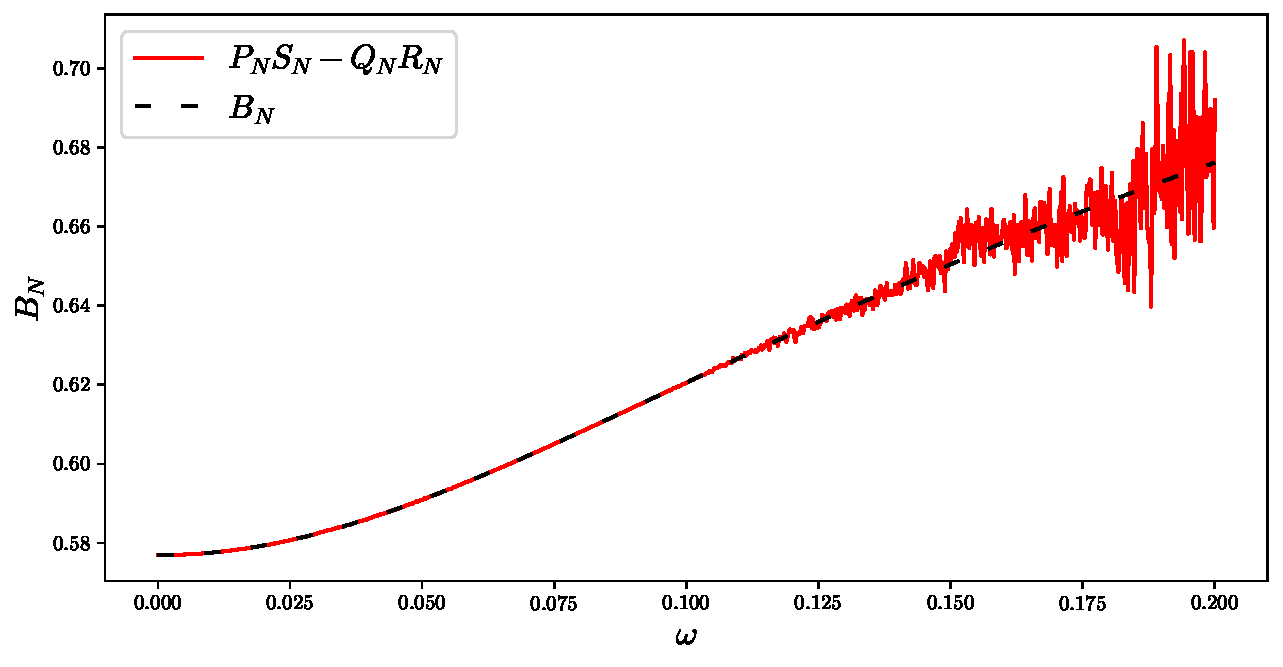
\includegraphics[width = \textwidth]{figs/det_identity_double_prec.pdf}
    \caption{Evaluation of the determinant of the Nevanlinna coefficients, $P_N S_N - Q_N R_N$, plotted against the theoretical value of the determinant, $B_N$. These Nevanlinna coefficients were determined at double precision using simulated data generated from a spectral function $\rho(\omega) = \delta(\omega - m_1) + \delta(\omega - m_2)$ with $am_1 = 0.05$ and $am_2 = 0.1$, using a lattice with temporal extent $\beta = 48$, and the first 20 nonzero Matsubara frequencies as input to the reconstruction algorithm. One can see that at large $\omega$ ($\omega \gtrsim 0.1$, the computed Nevanlinna determinant deviates from its theoretical value due to round-off error. }
    \label{fig:det_identity_double}
\end{figure}

\begin{figure}[!htp]
    \centering
    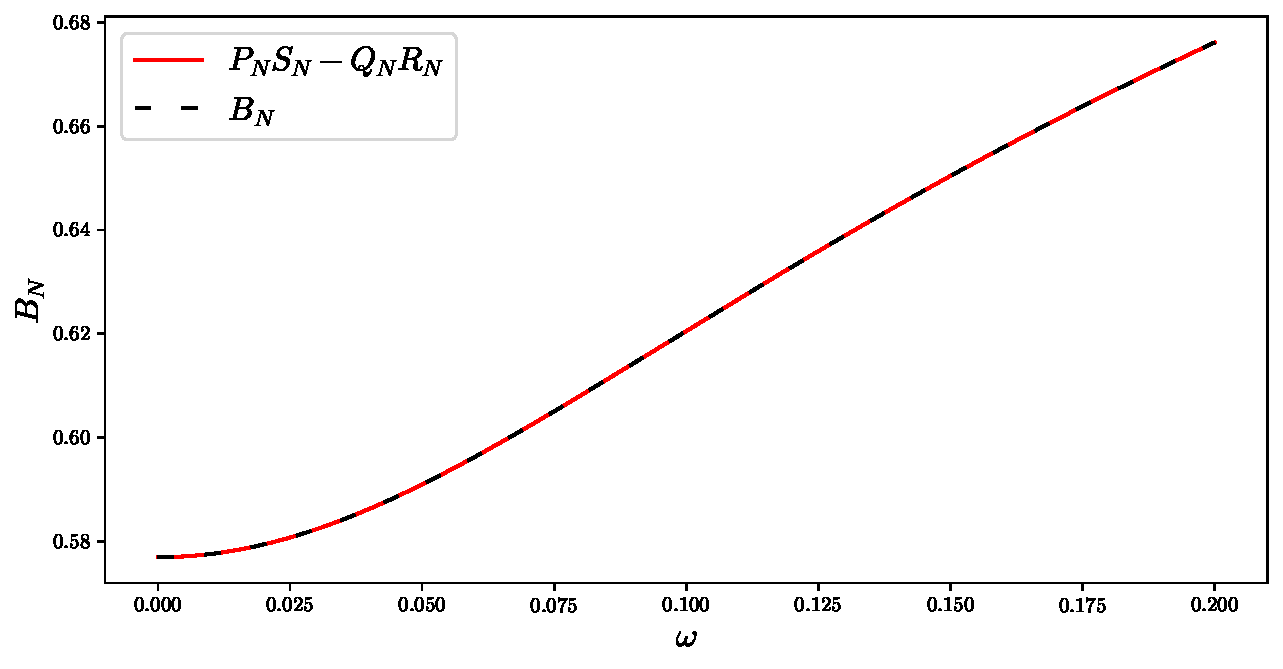
\includegraphics[width = \textwidth]{figs/det_identity_ext_prec.pdf}
    \caption{Same setup as Fig.~\ref{fig:det_identity_double}, but for 128-bits of precision. We observe that the extra precision allows us to verify Eq.~\eqref{eq:nevalinna_determinant} numerically, and we no longer observe the large deviations at $\omega\gtrsim 0.1$ due to round-off error.}
    \label{fig:det_identity_ext}
\end{figure}

The remarkable thing about this solution of the Nevanlinna-Pick problem is that there is an explicit description of the possible set of solutions to the problem in terms of the Nevanlinna coefficients. Recall that for any $f_N\in H^\infty$, the function,
\begin{equation}
    f = \frac{P_N f_N + Q_N}{R_N f_N + S_N}
    \label{eq:nev_pick_solution}
\end{equation}
solves the Nevanlinna-Pick interpolation problem. Conversely, \textbf{any solution} to the Nevanlinna-Pick interpolation problem may be parameterized as Eq.~\eqref{eq:nev_pick_solution} for some choice of $f_N\in H^\infty$. Varying $f_N$ over all possible functions in $H^\infty$ hence gives an envelope for $f$ which contains all possible solutions to the interpolation problem. 

The \textbf{wertevorrat} is defined as
\begin{equation}
    \Delta^{\mathbb D}(z) := \left\{ f(z) : f\in H^\infty \textnormal{ s.t. } \forall k,\, f(z_k) = w_k \right\}.
\end{equation}
\begin{theorem}
At fixed $z\in\mathbb D$, the wertevorrat is a \textbf{Euclidean disk} $\Delta^{\mathbb D}(z)\subseteq \mathbb D$ with center
\begin{equation}
    c_N(z) := \frac{P_N(z) \left( -\frac{R_N}{S_N}(z) \right)^* + Q_N(z)}{R_N(z) \left( -\frac{R_N}{S_N}(z) \right)^* + S_N(z)}
\end{equation}
and radius 
\begin{equation}
    r_N(z) := \frac{|B_N(z)|}{|S_N(z)|^2 - |R_N(z)|^2}.
\end{equation}
\end{theorem}

\begin{proof}
    TODO
\end{proof}

This is remarkable: it means that we have a direct measure of how ``ill-posed" the reconstruction problem is via the wertevorrat.

To reconstruct the spectral function $\rho_\eta(\omega) := \rho(z)$ at $z = \omega + i\eta$, we can thus determine the associated error in the spectral function $\delta\rho(z)$ by solving for the wertevorrat and mapping $\Delta^{\mathbb D}(z)$ back to $\mathbb C^+$. Define\footnote{Note that here $\Delta^{\mathbb D}(z)\subseteq\mathbb D$ is an open subset of the disk, and so $h^{-1}(\Delta(z))$ is not a function composition, but rather a \textit{pullback} of the domain $\Delta(z)$ by $h$.}
\begin{equation}
    \Delta(z) := C^{-1}(\Delta^{\mathbb D}(z)) \subseteq\mathbb C^+.
\end{equation}
As $h$ is continuous, $\Delta(z)$ is an open connected subset of $\mathbb C^+$. Let $\pi : \mathbb C^+\rightarrow \mathbb R$ be the projection onto the positive imaginary axis, i.e. $\pi(x + iy) := y$. Then the \textbf{error associated with the wertevorrat} is the interval in $\mathbb R$ defined as
\begin{equation}
    \delta\rho(z) := (\delta\rho^-(z), \delta\rho^+(z)) := \pi \left( \Delta(z) \right)
\end{equation}
where we use the fact that the projection $\pi$ maps the domain $\Delta(z)$ into an \textit{interval} $(\delta\rho^-(z), \delta\rho^+(z))$. The desired reconstruction envelope at each point may thus be quantified with
\begin{align}
    \delta\rho^-(z) = \inf \delta \rho(z) && \delta\rho^+(z) = \sup \delta \rho(z),
\end{align}
which are computed numerically by sampling $\partial\Delta^{\mathbb D}(z)$ uniformly with $N_{\mathrm{mesh}}\equiv 1000$ points, pulling each point back with $C^{-1}$ and projecting it onto its imaginary part with $\pi$ to sample from $\pi(\partial\Delta(z))$, and taking the maximum and minimum of this numerical estimate of  $\pi(\partial\Delta(z))$ to approximate $\delta\rho^-$ and $\delta\rho^+$. 

% The desired reconstruction envelope at each point $\omega$ is thus $(\delta\rho^-(\omega + i\eta), \delta\rho^+(\omega + i\eta))$. 

As the radius $r_N(z)$ of the disk must be positive, we see that for each $z\in\mathbb D$,
\begin{equation}
    |R_N(z)|\leq |S_N(z)|
\end{equation}

\subsection{SCRATCH: Closed form for the wertevorrat}

To determine $\delta\rho$, we parameterize the boundary of the wertevorrat as
\begin{equation}
    \partial \Delta(z) = \{ c_N(z) + r_N(z) e^{2\pi i t} : t\in [0, 1)\}.
\end{equation}
{\color{red}TODO $c_N$ may be IMAGINARY, have to take that into account}
The pullback of $\partial\Delta(z)$ by $h$ is thus parameterized as
\begin{equation}
    \partial \Gamma(z)[t] = h^{-1}(\partial\Delta(z)[t]) = i \left( \frac{1 + c_N + r_N e^{2\pi i t}}{1 - c_N - r_N e^{2\pi i t}} \right)
\end{equation}
which has imaginary part,
\begin{equation}
    \pi(\partial\Gamma(z))[t] = \frac{1 - c_N^2 - 2 c_N r_N \cos (2\pi t) - r_N^2}{(1 - c_N)^2 - 2 r_N (1 - c_N) \cos(2\pi t) + r_N^2}.
\end{equation}
To find $\delta\rho$, we must write $\pi(\partial\Gamma(z))$ as an interval $(\delta\rho^-(z), \delta\rho^+(z))$. The endpoints of this interval may only occur when the parameterization for $\pi(\partial\Gamma(z))[t]$ has a local extrema in $t$,
\begin{equation}
    \frac{d}{dt} \pi(\partial\Gamma(z))[t] = \frac{4\pi r_N (1 - c_N + r_N) (c_N + r_N - 1) \sin (2\pi t)}{ ( (1 - c_N)^2 - 2 r_N (1 - c) \cos(2\pi t)  + r_N^2  )^2} = 0
\end{equation}
which has solutions at $t = 0, \frac{1}{2}$; one solution is the minimum $\delta\rho^-(z)$, and the other solution is the maximum $\delta\rho^+(z)$. 
\begin{align}
    \frac{2}{1 - c_N - r_N} - 1 && \frac{2}{1 - c_N + r_N} - 1
\end{align}

% The error associated with the wertevorrat must be mapped back to $\mathbb C^+$ to determine $\delta\rho$. To do this, we parameter

{\color{red}TODO draw a figure of what's going on here.}

\subsection{Comparison between Ref.~\cite{fei2021nevanlinna} and Ref.\cite{https://doi.org/10.48550/arxiv.1405.3578}}

The major difference between our original procedure (Section~\ref{sec:nev_pick}) and Ref.~\cite{https://doi.org/10.48550/arxiv.1405.3578} is the domain of interpolation. In our case, the Schur algorithm is written out to reconstruct a contractive function $\Theta : \mathbb C^+\rightarrow\mathbb D$, while in the case of Ref.~\cite{https://doi.org/10.48550/arxiv.1405.3578}, the algorithm reconstructs a function on the disk, $f : \mathbb D\rightarrow\mathbb D$. These maps can be related with the commutative diagram,
\begin{equation}\begin{tikzcd}
	\mathbb C^+ \arrow[r, "h"] \arrow[dr, "\Theta"'] & \mathbb D\arrow[d, "f"] \\
	& \mathbb D.
\end{tikzcd}\end{equation}
We should be able to relate our respective quantities with $z_i = h(y_i)$. Because of this, there are a number of quantities that are good to have translated between the papers.

For the following list, we assume that the input Matsubara frequencies are $y_k = i\omega_k\in \mathbb C^+$, and the Nevanlinna Green's function data is $N_k\in\mathbb C^+$, with corresponding Mobi\"us transform $\lambda_k := h(N_k) \in\mathbb D$. The differences are as follows. 
\begin{itemize}
    \item Input frequencies. The frequencies $y_k\in\mathbb C^+$ are related to the points $\xi_k\in\mathbb D$ by Mobi\"us transformation:
    \begin{equation}
        \xi_k = h(y_k).
    \end{equation}
    \item Blaschke products: The two factors that we're using are similar in that they put the zeros in the correct places, but there are some definitional differences again related to the domain. Recall that for $a\in\mathbb D$ and $c\in\mathbb C^+$, we have
    \begin{align}
        b_a(z) = \frac{|a|}{a}\frac{a - z}{1 - a^* z} && \gamma_c(z) = \frac{z - c}{z - c^*},
    \end{align}
    where $b_a : \mathbb D\rightarrow\mathbb D$ and $\gamma_c : \mathbb C^+\rightarrow \mathbb D$. It is natural to ask if these maps are related via a Mobi\"us transformation, and indeed they are, at least for the case of interest when $c = y_i\in\mathbb C^+\cap \mathbb I = \mathbb I_{> 0}$ is a positive imaginary number (a Matsubara frequency). In this case, note that $h(c)^* = (\frac{z - i}{z + i})^* = \frac{-z+i}{-z-i} = h(c)$ is real\footnote{More intuitively, because the Mobi\"us transformation maps the positive imaginary axis to the midpoint of the disk $\mathbb D$ along the real axis.}, and in particular the phase $|h(c)| / h(c) = 1$. We have:
    \begin{align}
        \begin{split}
            b_{h(c)}(h(z)) &= \frac{h(c) - h(z)}{1 - h(c) h(z)} \\
            &= \frac{(c - i)(z + i) - (c + i)(z - i)}{(c + i)(z + i) - (c - i)(z - i)} \\
            &= - \frac{z - c}{z + c} \\
            &= - \gamma_c(z)
        \end{split}
    \end{align}
    % \begin{align}
    %     \begin{split}
    %         b_{h(c)}(h(z)) &= \frac{|h(c)|}{h(c)} \frac{h(c) - h(z)}{1 - h(c)^* h(z)} \\
    %         &= \frac{h(c) - h(z)}{1 - h(c) h(z)} \\
    %         &= \frac{\frac{c - i}{c + i} - \frac{z - i}{z + i}}{1 - \frac{c - i}{c + i} \frac{z - i}{z + i}} \\
    %         &= \frac{(c - i)(z + i) - (c + i)(z - i)}{(c + i)(z + i) - (c - i)(z - i)} \\
    %         &= - \frac{z - c}{z + c} \\
    %         &= - \gamma_c(z)
    %     \end{split}
    % \end{align}
    as $c^* = -c$. So, we see that the maps do commute, up to a negative sign:
    \begin{equation}\begin{tikzcd}
    	\mathbb C^+ \arrow[r, "h"] \arrow[dr, "-\gamma_{c}"'] & \mathbb D\arrow[d, "b_{h(c)}"] \\
    	& \mathbb D.
    \end{tikzcd}\end{equation}

    \item $\phi_k$ factors and $\theta_k$ matrices: Here we see that $\phi_k$ and $w_k^{(k-1)}$ play the same role, as well as $\theta_k$ and $U_k$. The defining equation for $w_k^{(k-1)}$ is to evaluate the $k^\mathrm{th}$ interpolant at $z_k$, i.e.
    \begin{align}
        w_k^{(k-1)} = f_{k-1}(\xi_k) && \phi_k = \theta_k(y_k; w)
    \end{align}
    The difference in the indexing for $f_{k-1}$ vs $\theta_k$ is that $f_{k-1}$ is expanded in terms of $U_k$, which is the equivalent of $\theta_k$ (up to normalization). So, we have:
    \begin{align}
        w_k^{(k-1)} = \phi_k && U_k = [\theta_{h(y_k)}\circ h]
        \label{eq:phik_wk_corr}
    \end{align}
    where the Mobi\"us transformations are applied to map each function to the correct domain. Note also that
    \begin{equation}
        \theta_{N+1} = f_N
    \end{equation}
    is the final contractive / $H^\infty$ function that is free to be chosen. 
    {\color{red}TODO does the $-$ sign on $\gamma_c = -b_{h(c)}\circ h$ do anything to this?}
    
    \item Nevanlinna coefficients: The Nevanlinna coefficients are defined as
    \begin{align}
        [\Theta_N] = \begin{pmatrix}
            a_N & b_N \\ c_N & d_N
        \end{pmatrix}
        &&
        U_1 ... U_N = \begin{pmatrix}
            P_N & Q_N \\ R_N & S_N
        \end{pmatrix}.
    \end{align}
    With the correspondence of Eq~\eqref{eq:phik_wk_corr}, we see that these are mostly the same, up to some applications of the Mobi\"us transformation. {\color{red}TODO work out the exact differences between each}
\end{itemize}
Note that in the code, we'll try to stay accurate to the notation of the paper we're adopting the algorithm from, just to make it more readable and match with these notes better. 

% \textbf{Scratch below this}

% \textbf{One major difference}: be careful about the domain of interpolation. We're reconstructing a contractive function $\theta : \mathbb C^+\rightarrow \mathbb D$, while the Nevanlinna-Pick papers are reconstructing a map on the unit disk $f : \mathbb D\rightarrow \mathbb D$. These maps can be related with the commutative diagram,
% \begin{equation}\begin{tikzcd}
% 	\mathbb C^+ \arrow[r, "h"] \arrow[dr, "\Theta"'] & \mathbb D\arrow[d, "f"] \\
% 	& \mathbb D
% \end{tikzcd}\end{equation}.
% We should be able to relate our respective quantities with $z_i = h(y_i)$. 

% Another important one:
% \begin{equation}
%     \phi_k := w_k^{(k-1)}
% \end{equation}
% since $\phi_k = \theta_k(\lambda_k)$, just like how $w_k^{(k-1)} = f_{k-1}(z_k)$, with the appropriate index substitution. 

% {\color{red}IMPORTANT}: Note that this may be why the Blaschke products look different: Blaschke products $b_a(z)$ are defined for $a\in\mathbb D$ as a map $b_a : \mathbb D\rightarrow \mathbb D$, whereas our $\gamma$ functions are defined as a map $\gamma : \mathbb C^+\rightarrow\mathbb D$, and should have some relation to $b_a\circ h$, where $h$ is the Mobius transform.

\section{Carlson's Theorem and Mathematical Considerations}
\label{sec:carleson}

In complex analysis, one learns that to analytically continue a function to the entire complex plane, it must first be defined on a dense subset of the plane.
This necessary and sufficient condition to define a unique analytic continuation can often be loosened.
One particular case of these conditions being loosened, which is exploited in our Nevanlinna-Pick method, is known as \textbf{Carlson's Theorem}. 
Roughly stated, Carlson's theorem says that if two functions $f$ and $g$ do not grow too fast\footnote{Here ``too fast'' mean that $f$ and $g$ grow sub-exponentially, i.e. there are parameters $C, \tau$ such that $f(z)\leq Ce^{-\tau|z|}$ as $|z|\rightarrow\infty$, and likewise for $g$.} as they approach $\infty$, and if then if $f(n) = g(n)$ on all non-negative integers $n\in\mathbb Z_+$, then $f(z) = g(z)$ for all $z\in\mathbb C$. 
In other words, assuming a function $f$ grows sub-exponentially\footnote{This behavior is true of all spectral functions, which must decay faster than a power law $\rho(\omega)\lesssim \omega^{-2}$~\cite{TODO}.}, then an analytic continuation of $f$ is defined as long as we specify $f$ on the integers. 
This is much more robust than the initial statement, since the integers are not a dense subset of the complex plane. 
One can loosen these requirements even further; Rubel proved in 1956 that if $f$ is defined on a subset $A\subseteq \{0, 1, 2, ...\}$  with upper density\footnote{The upper density $\rho(A)$ of a set $A$ is defined as \begin{equation}\rho(A) = \limsup \frac{|A\cap \{0, 1, ..., n - 1\}|}{n} .\end{equation}Essentially, this means that $A$ must contain most of the integers as $n\rightarrow\infty$, but it does not need to be the whole set. It needs to have an infinitely long ``tail''. } 1, then knowledge of a function's value on $A$ uniquely extends to the entire complex plane; in other words, as long as we know a spectral function's value on an infinite (but countable!) subset of the non-negative integers, we can recover the original function with analytic continuation. 

Carlson's theorem allows us to view the reconstruction problem in another way. Because we only know the retarded correlator at a finite number of Matsubara frequencies, we cannot apply the theorem; even with the strongest of analytic continuation theorems, we cannot form a unique analytic continuation. 

\section{Monte Carlo data and the Pick criterion}

\section{Results of Nevanlinna reconstructions}
\label{sec:nevanlinna_simulations}

\subsection{Simulated data and results}

\subsection{Monte Carlo data and results}

\section{Optimization techniques}


%\bibliography{spectral_fns}
\bibliography{spectral_functions}

\begin{appendices}

\newpage
%\onecolumngrid
\section{Hardy Spaces}
\label{app:complex_analysis}

For $1\leq p \leq \infty$, the \textbf{Hardy space $H^p$} is defined as the set of holomorphic functions on the disk $f : \mathbb D\rightarrow\mathbb D$ such that
\begin{equation}
    ||f||_p := \sup_{0 \leq r < 1} ||f_{r}||_{L^p(\mathbb T)} < \infty,
    \label{eq:hardy_space_dfn}
\end{equation}
where $f_{r}$ is the angular function defined on the unit circle $\mathbb T := \partial\mathbb D$ as
\begin{align}
    f_{r} : \mathbb T \rightarrow\mathbb D && f_{r}(e^{i\theta}) := f(re^{i\theta}).
\end{align}
The $L^p(\mathbb T)$-norm $||\cdot||_{L^p(\mathbb T)}$ for complex-valued functions $g : \mathbb T\rightarrow \mathbb C$ on $\mathbb T$ is defined for $1\leq p < \infty$ as
\begin{equation}
    ||g||_{L^p(\mathbb T)} := \left( \int_{\mathbb T} |g|^p dm \right)^{\frac{1}{p}} = \left( \frac{1}{2\pi} \int_{0}^{2\pi} |g(e^{i\theta})| d\theta \right)^{\frac{1}{p}},
\end{equation}
where $m$ is the normalized Lebesgue measure on $\mathbb T$, i.e. $dm(\theta) = d\theta / 2\pi$. For $p = \infty$, the p-norm is defined as the essential supremum of $|g|$,
\begin{equation}
    ||f||_{L^\infty(\mathbb T)} := \esssup_{\mathbb T}\, | g |, := \inf \{ a\in\mathbb R : |g| \leq a\;\mathrm{a.e.}\}
\end{equation}
where the essential supremum acts as a supremum except on sets of measure zero. 

For $1\leq p\leq \infty$, the definition (Eq.~\ref{eq:hardy_space_dfn}) of $H^p$ implies that for any $f\in H^p$, the radial limit of $f$,
\begin{equation}
    \tilde{f}(\theta) := \lim_{r\uparrow 1} f(re^{i\theta})
\end{equation}
exists a.e. as a map $\tilde{f} : \mathbb T\rightarrow \mathbb D$ and is finite, with $L^p(\mathbb T)$ norm
\begin{equation}
    ||\tilde{f}||_{L^p(\mathbb T)} = ||f||_p. 
\end{equation}
The function $f$ may be obtained from its radial limit $\tilde{f}$ by convolution,
\begin{equation}
    f(re^{i\theta}) = P_r * \tilde f := \int_{\mathbb T} P_r(t - \theta) \tilde f(e^{it})\, dm(t) = \frac{1}{2\pi} \int_{0}^{2\pi} P_{r}(t - \theta) \tilde f(e^{it})\, dt,
\end{equation}
where $P_r(\theta)$ is the \textbf{Poisson kernel},
\begin{equation}
    P_r(\theta) := \frac{1 - r^2}{|1 - re^{i\theta}|^2}. 
\end{equation}
Note that because the map $[1, \infty]\ni p \mapsto ||f||_p$ is non-decreasing for any $f\in\mathrm{Hol}{\mathbb D}$, we have the increasing tower $H^\infty \subseteq H^p \subseteq H^q \subseteq H^1$ for any $1\leq q\leq p\leq \infty$. 
% Note that Fatou's theorem is stronger and implies convergence of $f$ to $\tilde f$ as $r\rightarrow\infty$ in a stronger way than the radial limit, instead as a ``non-tangential limit" across a Stoltz angle. 

The next notion to introduce is that of inner and outer functions. We say that $f\in H^\infty$ is an \textbf{inner function} if $1\tilde{f}(e^{i\theta})| = 1$ for almost every $e^{i\theta}\in\mathbb T$. The definition of an outer function is more complicated. For a measurable function $h$ on $\mathbb T$ with $\log |h|\in\mathbb T$, we define
\begin{equation}
    [h](z) := \exp \left( \int_{\mathbb T} \frac{\zeta + z}{\zeta - z} \log |h(\zeta)|\, dm(\zeta) \right)
\end{equation}
for each $z\in\mathbb D$, and we say that $f\in H^1$ is an \textbf{outer function} if it may be written as
\begin{equation}
    f = \lambda [h]
\end{equation}
for some measurable $h$ and some $\lambda\in\mathbb T$. Outer functions have no zeros in $\mathbb D$ because of the $\exp$ baked into their definition. 
% https://math.stackexchange.com/questions/2594569/definition-of-smirnov-class

% Inner-outer factorization

The \textbf{Smirnov class} of functions on the disk is defined as
\begin{equation}
    \mathcal S := \left\{ f\in\mathrm{Hol}(\mathbb D) : f = \frac{f_1}{f_2} \textnormal{ with } f_1, f_2\in\bigcup_{p = 1}^\infty H^p \textnormal{ and $f_2$ is outer} \right\}.
\end{equation}
where $\mathrm{Hol}(\mathbb D)$ is the space of holomorphic functions $\mathbb D \rightarrow\mathbb D$. 

% A function $f\in H^1$ is an \textbf{outer function} if for each $z\in\mathbb D$, we have
%$re^{i\theta}\in\mathbb D$ it may be written as
% \begin{equation}
%     f(re^{i\theta}) = \alpha \exp\left( \frac{1}{2\pi} \int_0^{2\pi} \frac{e^{it} + re^{i\theta}}{e^{it} - re^{i\theta}} k(e^{it})\, dt \right)
% \end{equation}
% for some real-valued integrable function $k$, with $\alpha\in\mathbb T$. 

% Want to get to Smirnov classes

% \begin{equation}
%     ||f||_p := \sup_{0\leq r < 1} \left( \frac{1}{2\pi} \int_0^{2\pi} |f(re^{i\theta})|^p\,d\theta \right)^{\frac{1}{p}}
% \end{equation}
% exists and is finite. For $p = \infty$, the \textbf{Hardy space $H^\infty$} is defined as the set of functions $f : \mathbb D\rightarrow\mathbb D$ whose 

\section{Matrix-vector notation for continued fractions}

The continued fractions expansion used in this writeup are often denoted with a matrix-vector multiplication, and it remains to show that this notation is well-defined. Consider the following expansion:
\begin{align}
    f = \frac{b_1 f_1 + w_1}{w_1^* b_1 f_1 + 1} =: U_1 f_1 &&
    U_k := \frac{1}{\sqrt{1 - |w_k|^2}} \begin{pmatrix}
        b_k & w_k \\ w_k^* b_k & 1
    \end{pmatrix}
    \label{eq:matrix_vector_notation}
\end{align}
where $b_k := b_{\xi_k}$ is the Blaschke factor with zero $\{\xi_k\}$, and we are suppressing the $(k-1)$ superscript of $w_k^{(k-1)}$. We also regard $f_1$ in the above equation as the column vector $f_1 \rightarrow \begin{pmatrix}
    f_1 & 1
\end{pmatrix}^T$. 

To make this notation well-defined, we must define matrix multiplication and inversion, and show that matrix-matrix and matrix-vector products yield the equivalent function compositions. Here are the important points:
\begin{enumerate}
    \item As in the case of $f_1 \rightarrow\begin{pmatrix} f_1 & 1 \end{pmatrix}^T$, we regard functions $f$ as column vectors, whose top component is their numerator and whose bottom component is their denominator. In this way, matrix-vector multiplication gives us what we want; consider explicitly writing out Eq.~\eqref{eq:matrix_vector_notation}:
    \begin{equation}
        \begin{pmatrix}
            \mathrm{num}(f) \\ \mathrm{denom}(f)
        \end{pmatrix} = \frac{1}{\sqrt{1 - |w_1|^2}}\begin{pmatrix}
            b_1 & w_1 \\ w_1^* b_1 & 1
        \end{pmatrix} \begin{pmatrix} f_1 \\ 1 \end{pmatrix} = \frac{1}{\sqrt{1 - |w_1|^2}}\begin{pmatrix}
            b_1 f_1 + w_1 \\ w_1^* b_1 f_1 + 1
        \end{pmatrix}
        \label{eq:num_denom_expansion}
    \end{equation} 

    \item Scalar multiplication of a matrix $U_k$ by $a\neq 0$ \textbf{does not change its action on functions} in this notation. This is because if $U_k\rightarrow a U_k$, this multiplies both the numerator and the denominator of the resulting matrix-vector product by $a$, which cancels out. Note that in Eq.~\eqref{eq:num_denom_expansion}, $\sqrt{1 - |w_k|^2}$ doesn't affect the final value of $f$. 

    \item Matrix-matrix multiplication preserves function composition. Consider evaluating $U_1 U_2 f$, where the expansion of $f$ in terms of $f_2$ is
    \begin{equation}
        f = \frac{b_1 \frac{b_2 f_2 + w_2}{w_2^* b_2 f_2 + 1} + w_1}{ w_1^* b_1 \frac{b_2 f_2 + w_2}{w_2^* b_2 f_2 + 1} + 1} = \frac{b_1 b_2 f_2 + b_1 w_2 + b_2 w_1 w_2^* f_2 + w_1}{b_1 b_2 w_1^* f_2 + b_1 w_1^* w_2 + b_2 w_2^* f_2 + 1}.
        \label{eq:f_expansion_app}
    \end{equation}
    For the notation to be well-defined, $U_1 U_2 f_2$ must equal this value. We have:
    \begin{align}\begin{split}
        U_1 U_2 f_2 &= N \begin{pmatrix}
        b_1 & w_1 \\ w_1^* b_1 & 1
    \end{pmatrix}
    \begin{pmatrix}
        b_2 & w_2 \\ w_2^* b_2 & 1
    \end{pmatrix}
    \begin{pmatrix}
        f_2 \\ 1
    \end{pmatrix}
    = 
    N \begin{pmatrix}
        b_1 & w_1 \\ w_1^* b_1 & 1
    \end{pmatrix} \begin{pmatrix}
        f_2 b_2 + w_2 \\
        w_2^* b_2 f_2 + 1
    \end{pmatrix} \\
    &= N \begin{pmatrix}
        b_1 b_2 f_2 + b_1 w_2 +  b_2 w_1 w_2^* f_2 + w_1 \\
        b_1 b_2 w_1^* f_2  + b_1 w_1^* w_2 + b_2 w_2^* f_2 + 1
    \end{pmatrix}
    \end{split}\end{align}
    where $N = 1 / (\sqrt{(1 - |w_1|^2) (1 - |w_2|^2)}$ is a normalization that does not affect the outcome. We see this exactly yields Eq.~\eqref{eq:f_expansion_app}.

    \item Matrix inversion: The last order of business is to make sure we can invert these matrices in a consistent way. Recall the inverse of $U_k$ is
    \begin{equation}
        U_k^{-1} = \frac{1}{b_k} \frac{1}{\sqrt{1 - |w_k|^2}} \begin{pmatrix}
            1 & -w_k \\ -w_k^* b_k & b_k. 
        \end{pmatrix}
    \end{equation}
    To guarantee everything is consistent, we will apply $U_k^{-1}$ to $f$ to extract $f_1$. We should obtain the corresponding solution:
    \begin{equation}
        f = \frac{b_1 f_1 + w_1}{w_1^* b_1 f_1 + 1} \implies f_1 = \frac{w_1 - f}{w_1^* b_1 f - b_1} = \frac{f - w_1}{b_1 - w_1^* b_1 f}.
    \end{equation}
    On the matrix inverse side, we have:
    \begin{equation}
        U_1^{-1} f = N \begin{pmatrix}
            1 & -w_1 \\ -w_1^* b_1 & b_1
        \end{pmatrix} \begin{pmatrix}
            f \\ 1
        \end{pmatrix} = N \begin{pmatrix}
            f - w_1 \\ -w_1^* b_1 f + b_1
        \end{pmatrix}
    \end{equation}
    which is exactly what we wanted.
    
\end{enumerate}

\newpage
\section{Blaschke Products}
\label{app:blaschke}

For a given set of points $\{\xi_k\}$, the Blaschke factors $b_k(z)$ and their product $B_N(z)$,
\begin{align}
    b_k(z)\equiv \frac{|\xi_k|}{\xi_k} \frac{\xi_k - z}{1 - \xi_k^* z} && B_N(z) \equiv \prod_{k = 1}^N b_{k}(z)
\end{align}
are interesting to study in their own right~\cite{blaschke_products_book}, as their properties inform many properties of the Nevanlinna coefficients $P_N, Q_N, R_N,$ and $S_N$. Note that the points where the interpolation problem is fixed, $\xi_k$, all lie on the real axis in $\mathbb D$,
\begin{equation}
    \xi_k = h(i\omega_k)\in\mathbb D\cap \mathbb R
\end{equation}
since the Matsubara frequencies are purely imaginary. With this simplification, the phase factor can be neglected,
\begin{equation}
    b_k(z) = \frac{\xi_k - z}{1 - \xi_k z}.
\end{equation}

There are two main regions to consider $b_k$ and $B_N$: on the real axis of $\mathbb D$, and as we approach the boundary of $\mathbb D$. In the first case, note that by construction, $b_k(z)$ must vanish as we approach $\xi_k$, hence we expect $B_N(z)$ to have $N$ zeros at $\{\xi_k\}_{k = 1}^N$. Fig.~\ref{fig:blaschke_real_axis} shows the Mobi\"us transform of the first 20 nonzero Matsubara frequencies, $\xi_k$, on a lattice with $\beta = 48$, along with the corresponding Blaschke factors $b_k$ and the Blaschke product $B_N$. Note that each $b_k$ vanishes at the corresponding $\xi_k$. The Blaschke product $B_N$ is very small in the bulk of the disk $\mathbb D$, but approaches 1 at the boundary of the disk, $\partial\mathbb D$. 

\begin{figure}[!htp]
    \centering
    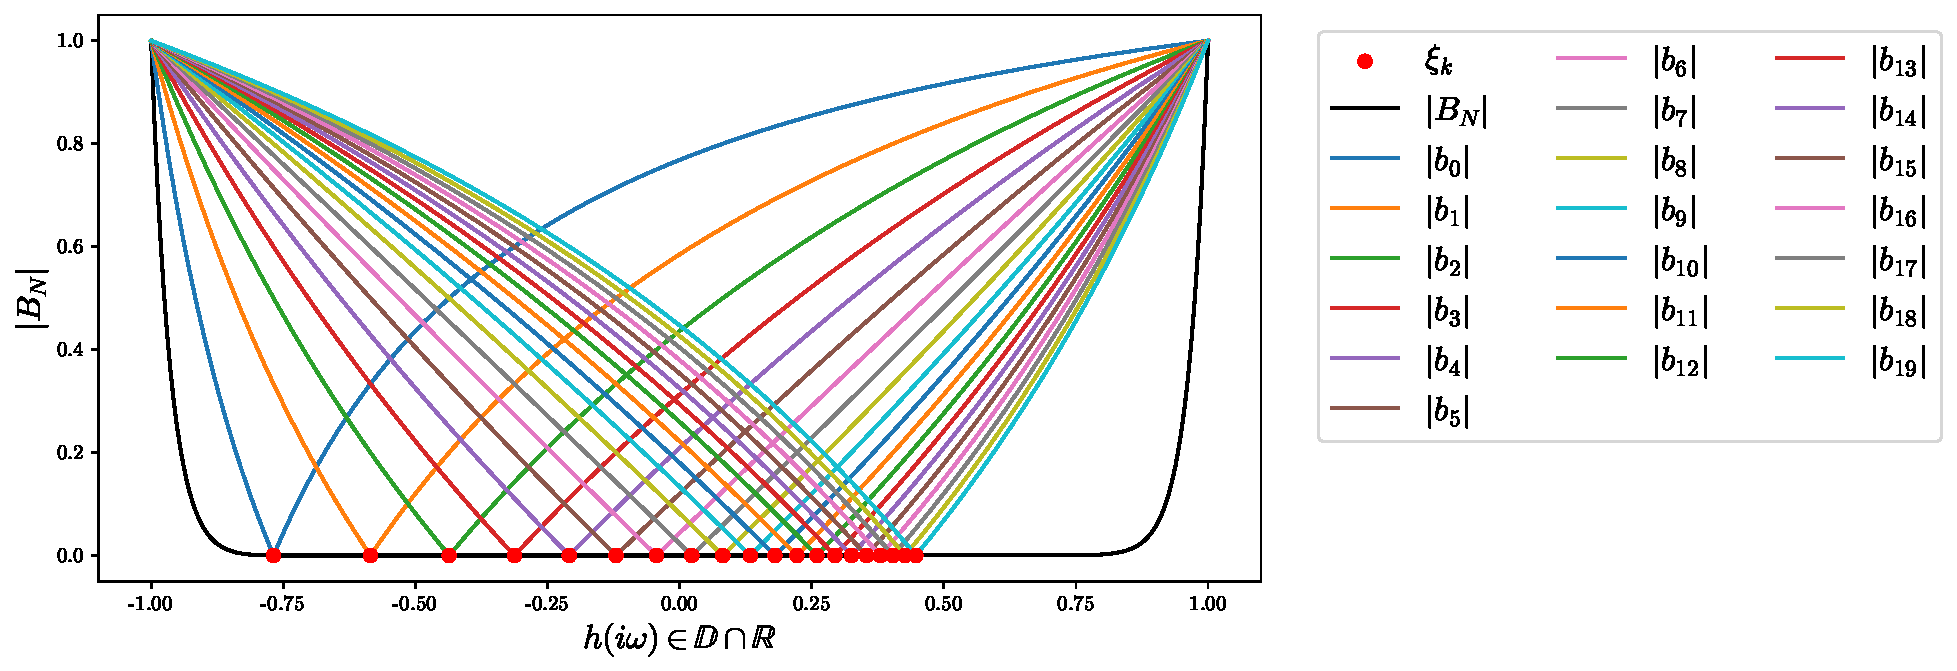
\includegraphics[width = \textwidth]{figs/blashke_real_axis.pdf}
    \caption{Evaluation of the Blaschke factors and the Blaschke product on the real axis of the disk, $\mathbb D\cap \mathbb R$. The Mobi\"us transform of the Matsubara frequencies, $\xi_k$, are shown in red, while the Blaschke product $B_N$ is the black curve, and the colored curves are the corresponding Blaschke factors $b_k$. The depicted Matsubara frequencies are the first 20 non-zero frequencies on a lattice with temporal extent $\beta = 48$. }
    \label{fig:blaschke_real_axis}
\end{figure}

The fact that $B_N(z)\rightarrow 1$ as $z\rightarrow \mathbb D$ is not a coincidence, and can be seen by considering the behavior of each Blaschke factor $b_k(z)$ as one approaches $\partial \mathbb D$. As $z\rightarrow e^{i\alpha}\in\partial\mathbb D$, one can expand out the individual Blaschke product $b_k(z)$ as
\begin{equation}
    b_k(z) \rightarrow \frac{\xi_k - e^{i\alpha}}{1 - \xi_k e^{i\alpha}} \left( \frac{1 + \xi_k e^{-i\alpha}}{1 + \xi_k e^{-i\alpha}} \right) = e^{-i\alpha} \left( \frac{\xi_k^2 - 1}{1 - 2\xi_k \sin\alpha - \xi_k^2} \right).
\end{equation}
Note that $\alpha = 0$ corresponds to evaluation of the Blaschke factor on the real axis, as in Fig.~\ref{fig:blaschke_real_axis}, and we see that $|b_k(z)|\rightarrow 1$ in this case, as is depicted in the data. 

What does $B_N(z)$ look like for $\alpha\neq 0$? We can prove a general bound with the (reverse) triangle inequality,
\begin{equation}
    |b_k(z)| = \left| \frac{\xi_k - z}{1 - \xi_k z} \right| \geq \frac{||z| - |\xi_k||}{1 + |\xi_k z|} \xrightarrow{|z|\rightarrow 1} \frac{1 - |\xi_k|}{1  + |\xi_k|}. 
\end{equation}
If we plot the Blaschke factors on an evaluation contour $h(\omega + i\eta)$, we can numerically study its behavior. We see that as we approach $1\in\mathbb D$ (equivalently, $\omega\rightarrow\infty$ where $\omega + i\eta\in\mathbb C^+$ is the domain of the Matsubara frequencies), the Blaschke factors all approach 1, while as we approach $-1\in\mathbb D$ (equivalently, $\omega\rightarrow 0$) the Blaschke factors do not approach 1 at fixed $\eta$. However, varying $\eta$ and sending $\eta\downarrow 0$  sends each Blaschke factor to 1 asymptotically ({\color{red}TODO prove this?})

\begin{figure}[!htp]
    \centering
    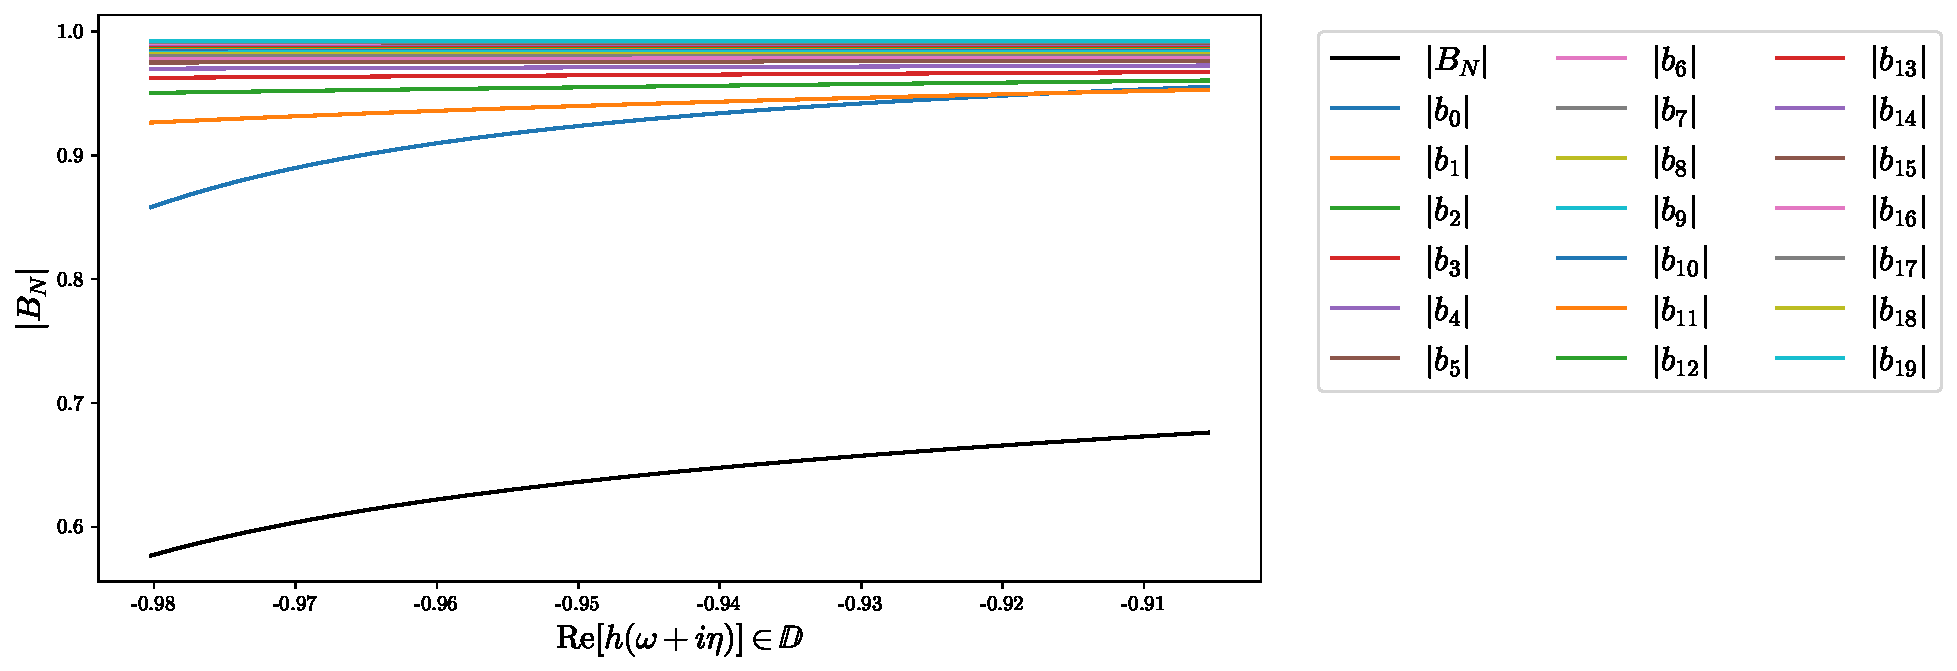
\includegraphics[width = \textwidth]{figs/blashke_eval_axis.pdf}
    \caption{Blaschke factors evaluated on the evaluation contour $h(\omega + i\eta)\in\mathbb D$, for $\omega\in [0, 2]$ and $\eta = 0.01$. The further $\xi_k$ is from the boundary of the disk, the closer $b_k$ remains to 1.}
    \label{fig:blaschke_eval_axis}
\end{figure}

\begin{figure}[!htp]
    \centering
    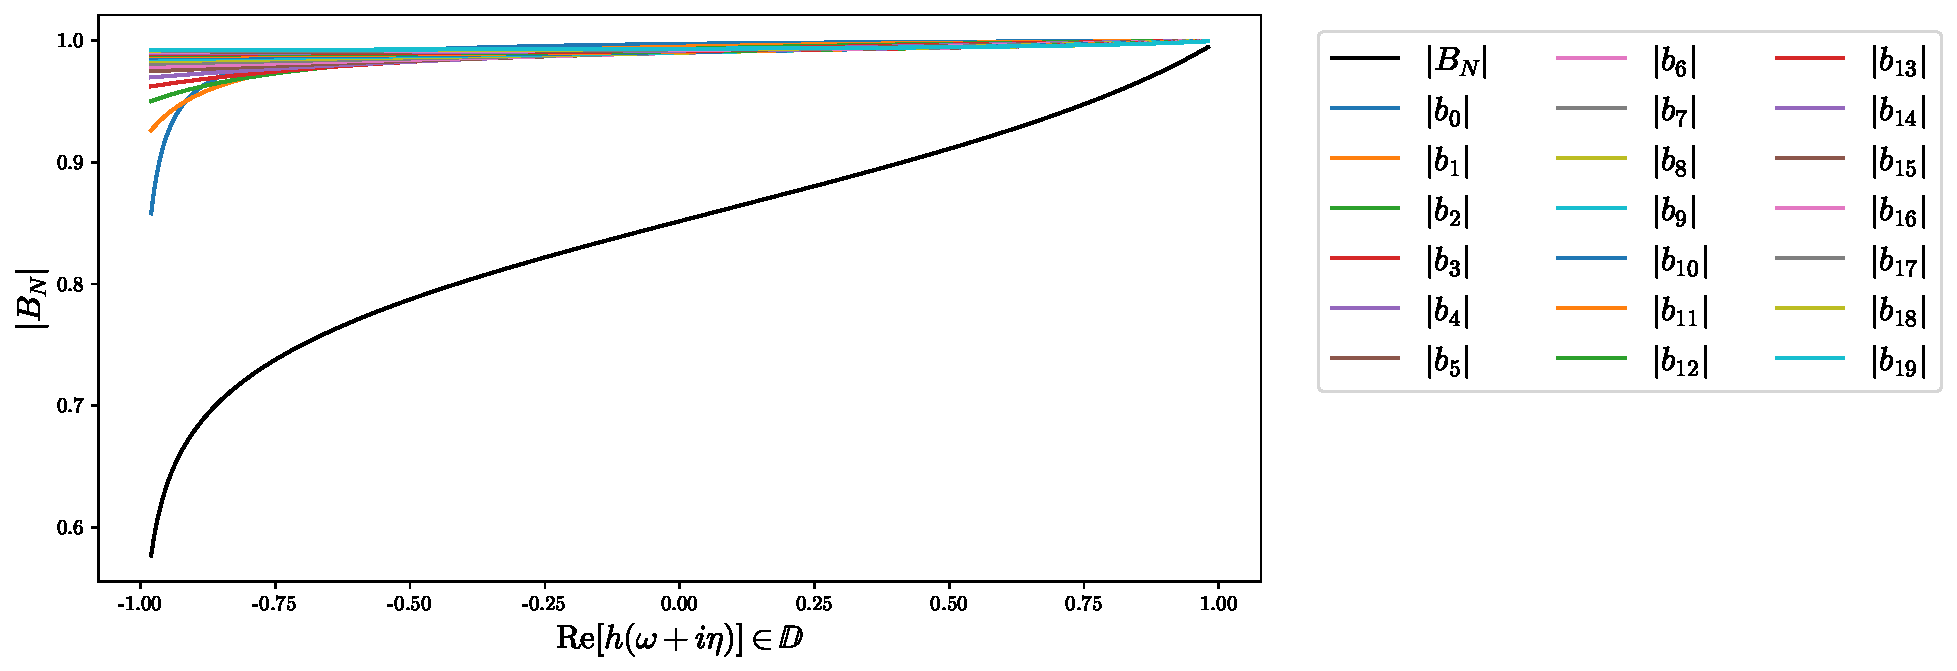
\includegraphics[width = \textwidth]{figs/blashke_eval_axis_full.pdf}
    \caption{Blaschke factors evaluated on a larger evaluation contour, $h(\omega + i\eta)\in\mathbb D$ for $\omega\in [0, 100]$ and $\eta = 0.01$. This corresponds to a contour on the lower half of $\mathbb D$, near the boundary of the disk, running from $-1$ to almost $+1$. Fig.~\ref{fig:blaschke_eval_axis} corresponds to the cross section of this plot that approximately has $h(\omega + i\eta)\in [0.98 to 0.91]$.}
    \label{fig:blaschke_eval_axis_full}
\end{figure}

\end{appendices}

\end{document}